\documentclass[twoside]{book}

% Packages required by doxygen
\usepackage{fixltx2e}
\usepackage{calc}
\usepackage{doxygen}
\usepackage[export]{adjustbox} % also loads graphicx
\usepackage{graphicx}
\usepackage[utf8]{inputenc}
\usepackage{makeidx}
\usepackage{multicol}
\usepackage{multirow}
\PassOptionsToPackage{warn}{textcomp}
\usepackage{textcomp}
\usepackage[nointegrals]{wasysym}
\usepackage[table]{xcolor}

% Font selection
\usepackage[T1]{fontenc}
\usepackage[scaled=.90]{helvet}
\usepackage{courier}
\usepackage{amssymb}
\usepackage{sectsty}
\renewcommand{\familydefault}{\sfdefault}
\allsectionsfont{%
  \fontseries{bc}\selectfont%
  \color{darkgray}%
}
\renewcommand{\DoxyLabelFont}{%
  \fontseries{bc}\selectfont%
  \color{darkgray}%
}
\newcommand{\+}{\discretionary{\mbox{\scriptsize$\hookleftarrow$}}{}{}}

% Page & text layout
\usepackage{geometry}
\geometry{%
  a4paper,%
  top=2.5cm,%
  bottom=2.5cm,%
  left=2.5cm,%
  right=2.5cm%
}
\tolerance=750
\hfuzz=15pt
\hbadness=750
\setlength{\emergencystretch}{15pt}
\setlength{\parindent}{0cm}
\setlength{\parskip}{3ex plus 2ex minus 2ex}
\makeatletter
\renewcommand{\paragraph}{%
  \@startsection{paragraph}{4}{0ex}{-1.0ex}{1.0ex}{%
    \normalfont\normalsize\bfseries\SS@parafont%
  }%
}
\renewcommand{\subparagraph}{%
  \@startsection{subparagraph}{5}{0ex}{-1.0ex}{1.0ex}{%
    \normalfont\normalsize\bfseries\SS@subparafont%
  }%
}
\makeatother

% Headers & footers
\usepackage{fancyhdr}
\pagestyle{fancyplain}
\fancyhead[LE]{\fancyplain{}{\bfseries\thepage}}
\fancyhead[CE]{\fancyplain{}{}}
\fancyhead[RE]{\fancyplain{}{\bfseries\leftmark}}
\fancyhead[LO]{\fancyplain{}{\bfseries\rightmark}}
\fancyhead[CO]{\fancyplain{}{}}
\fancyhead[RO]{\fancyplain{}{\bfseries\thepage}}
\fancyfoot[LE]{\fancyplain{}{}}
\fancyfoot[CE]{\fancyplain{}{}}
\fancyfoot[RE]{\fancyplain{}{\bfseries\scriptsize Generated by Doxygen }}
\fancyfoot[LO]{\fancyplain{}{\bfseries\scriptsize Generated by Doxygen }}
\fancyfoot[CO]{\fancyplain{}{}}
\fancyfoot[RO]{\fancyplain{}{}}
\renewcommand{\footrulewidth}{0.4pt}
\renewcommand{\chaptermark}[1]{%
  \markboth{#1}{}%
}
\renewcommand{\sectionmark}[1]{%
  \markright{\thesection\ #1}%
}

% Indices & bibliography
\usepackage{natbib}
\usepackage[titles]{tocloft}
\setcounter{tocdepth}{3}
\setcounter{secnumdepth}{5}
\makeindex

% Hyperlinks (required, but should be loaded last)
\usepackage{ifpdf}
\ifpdf
  \usepackage[pdftex,pagebackref=true]{hyperref}
\else
  \usepackage[ps2pdf,pagebackref=true]{hyperref}
\fi
\hypersetup{%
  colorlinks=true,%
  linkcolor=blue,%
  citecolor=blue,%
  unicode%
}

% Custom commands
\newcommand{\clearemptydoublepage}{%
  \newpage{\pagestyle{empty}\cleardoublepage}%
}

\usepackage{caption}
\captionsetup{labelsep=space,justification=centering,font={bf},singlelinecheck=off,skip=4pt,position=top}

%===== C O N T E N T S =====

\begin{document}

% Titlepage & ToC
\hypersetup{pageanchor=false,
             bookmarksnumbered=true,
             pdfencoding=unicode
            }
\pagenumbering{alph}
\begin{titlepage}
\vspace*{7cm}
\begin{center}%
{\Large Markov-\/master code documentation }\\
\vspace*{1cm}
{\large Generated by Doxygen 1.8.14}\\
\end{center}
\end{titlepage}
\clearemptydoublepage
\pagenumbering{roman}
\tableofcontents
\clearemptydoublepage
\pagenumbering{arabic}
\hypersetup{pageanchor=true}

%--- Begin generated contents ---
\chapter{license}
\label{md__d_1__jacob__d__documents__c_o_m_p_8045__game_2_backup__c_o_m_p_8045__game_2__out_of__assets-3a47f7332cdad394570548c193657856}
\Hypertarget{md__d_1__jacob__d__documents__c_o_m_p_8045__game_2_backup__c_o_m_p_8045__game_2__out_of__assets-3a47f7332cdad394570548c193657856}
Copyright © 2018 John Gietzen

Permission is hereby granted, free of charge, to any person obtaining a copy of this software and associated documentation files (the \char`\"{}\+Software\char`\"{}), to deal in the Software without restriction, including without limitation the rights to use, copy, modify, merge, publish, distribute, sublicense, and/or sell copies of the Software, and to permit persons to whom the Software is furnished to do so, subject to the following conditions\+:

The above copyright notice and this permission notice shall be included in all copies or substantial portions of the Software.

T\+HE S\+O\+F\+T\+W\+A\+RE IS P\+R\+O\+V\+I\+D\+ED \char`\"{}\+A\+S I\+S\char`\"{}, W\+I\+T\+H\+O\+UT W\+A\+R\+R\+A\+N\+TY OF A\+NY K\+I\+ND, E\+X\+P\+R\+E\+SS OR I\+M\+P\+L\+I\+ED, I\+N\+C\+L\+U\+D\+I\+NG B\+UT N\+OT L\+I\+M\+I\+T\+ED TO T\+HE W\+A\+R\+R\+A\+N\+T\+I\+ES OF M\+E\+R\+C\+H\+A\+N\+T\+A\+B\+I\+L\+I\+TY, F\+I\+T\+N\+E\+SS F\+OR A P\+A\+R\+T\+I\+C\+U\+L\+AR P\+U\+R\+P\+O\+SE A\+ND N\+O\+N\+I\+N\+F\+R\+I\+N\+G\+E\+M\+E\+NT. IN NO E\+V\+E\+NT S\+H\+A\+LL T\+HE A\+U\+T\+H\+O\+RS OR C\+O\+P\+Y\+R\+I\+G\+HT H\+O\+L\+D\+E\+RS BE L\+I\+A\+B\+LE F\+OR A\+NY C\+L\+A\+IM, D\+A\+M\+A\+G\+ES OR O\+T\+H\+ER L\+I\+A\+B\+I\+L\+I\+TY, W\+H\+E\+T\+H\+ER IN AN A\+C\+T\+I\+ON OF C\+O\+N\+T\+R\+A\+CT, T\+O\+RT OR O\+T\+H\+E\+R\+W\+I\+SE, A\+R\+I\+S\+I\+NG F\+R\+OM, O\+UT OF OR IN C\+O\+N\+N\+E\+C\+T\+I\+ON W\+I\+TH T\+HE S\+O\+F\+T\+W\+A\+RE OR T\+HE U\+SE OR O\+T\+H\+ER D\+E\+A\+L\+I\+N\+GS IN T\+HE S\+O\+F\+T\+W\+A\+RE. 
\chapter{Markov}
\label{md__d_1__jacob__d__documents__c_o_m_p_8045__game_2_backup__c_o_m_p_8045__game_2__out_of__assets-edb80a0995ee52d9aeb49a028bbe9151}
\Hypertarget{md__d_1__jacob__d__documents__c_o_m_p_8045__game_2_backup__c_o_m_p_8045__game_2__out_of__assets-edb80a0995ee52d9aeb49a028bbe9151}
\mbox{\hyperlink{license_8md}{!\mbox{[}M\+IT Licensed\mbox{]}(https\+://img.shields.io/badge/license-\/\+M\+I\+T-\/blue.svg?style=flat-\/square)}} \href{http://nuget.org/packages/Markov}{\tt }

\href{https://ci.appveyor.com/project/otac0n/Markov}{\tt } \href{https://codecov.io/gh/otac0n/Markov}{\tt } \href{http://nuget.org/packages/Markov}{\tt }

\subsection*{Getting Started }

\begin{DoxyVerb}PM> Install-Package Markov
\end{DoxyVerb}


For details getting started, please see the \href{https://github.com/otac0n/markov/wiki/Getting-Started}{\tt Getting Started Guide} 
\chapter{Namespace Index}
\section{Packages}
Here are the packages with brief descriptions (if available)\+:\begin{DoxyCompactList}
\item\contentsline{section}{\mbox{\hyperlink{namespace_markov}{Markov}} }{\pageref{namespace_markov}}{}
\item\contentsline{section}{\mbox{\hyperlink{namespace_markov_1_1_tests}{Markov.\+Tests}} }{\pageref{namespace_markov_1_1_tests}}{}
\end{DoxyCompactList}

\chapter{Hierarchical Index}
\section{Class Hierarchy}
This inheritance list is sorted roughly, but not completely, alphabetically\+:\begin{DoxyCompactList}
\item \contentsline{section}{Markov.\+Tests.\+Chain\+State\+Tests}{\pageref{class_markov_1_1_tests_1_1_chain_state_tests}}{}
\item I\+Equatable$<$ Chain\+State$<$ T $>$$>$\begin{DoxyCompactList}
\item \contentsline{section}{Markov.\+Chain\+State$<$ T $>$}{\pageref{class_markov_1_1_chain_state}}{}
\end{DoxyCompactList}
\item I\+List\begin{DoxyCompactList}
\item \contentsline{section}{Markov.\+Chain\+State$<$ T $>$}{\pageref{class_markov_1_1_chain_state}}{}
\end{DoxyCompactList}
\item \contentsline{section}{Markov.\+Markov\+Chain$<$ T $>$}{\pageref{class_markov_1_1_markov_chain}}{}
\item \contentsline{section}{Markov.\+Tests.\+Markov\+Chain\+Tests}{\pageref{class_markov_1_1_tests_1_1_markov_chain_tests}}{}
\end{DoxyCompactList}

\chapter{Class Index}
\section{Class List}
Here are the classes, structs, unions and interfaces with brief descriptions\+:\begin{DoxyCompactList}
\item\contentsline{section}{\mbox{\hyperlink{class_markov_1_1_chain_state}{Markov.\+Chain\+State$<$ T $>$}} \\*Represents a state in a \mbox{\hyperlink{namespace_markov}{Markov}} chain. }{\pageref{class_markov_1_1_chain_state}}{}
\item\contentsline{section}{\mbox{\hyperlink{class_markov_1_1_tests_1_1_chain_state_tests}{Markov.\+Tests.\+Chain\+State\+Tests}} }{\pageref{class_markov_1_1_tests_1_1_chain_state_tests}}{}
\item\contentsline{section}{\mbox{\hyperlink{class_markov_1_1_markov_chain}{Markov.\+Markov\+Chain$<$ T $>$}} \\*Builds and walks interconnected states based on a weighted probability. }{\pageref{class_markov_1_1_markov_chain}}{}
\item\contentsline{section}{\mbox{\hyperlink{class_markov_1_1_tests_1_1_markov_chain_tests}{Markov.\+Tests.\+Markov\+Chain\+Tests}} }{\pageref{class_markov_1_1_tests_1_1_markov_chain_tests}}{}
\end{DoxyCompactList}

\chapter{File Index}
\section{File List}
Here is a list of all files with brief descriptions\+:\begin{DoxyCompactList}
\item\contentsline{section}{D\+:/\+Jacob\+\_\+\+D/\+Documents/\+C\+O\+M\+P 8045 Game 2 backup/\+C\+O\+M\+P 8045 Game 2/\+Out of Assets-\/ofmarkov-\/master/markov-\/master/\+Markov.\+Tests/\mbox{\hyperlink{_chain_state_tests_8cs}{Chain\+State\+Tests.\+cs}} }{\pageref{_chain_state_tests_8cs}}{}
\item\contentsline{section}{D\+:/\+Jacob\+\_\+\+D/\+Documents/\+C\+O\+M\+P 8045 Game 2 backup/\+C\+O\+M\+P 8045 Game 2/\+Out of Assets-\/ofmarkov-\/master/markov-\/master/\+Markov.\+Tests/\mbox{\hyperlink{_markov_chain_tests_8cs}{Markov\+Chain\+Tests.\+cs}} }{\pageref{_markov_chain_tests_8cs}}{}
\item\contentsline{section}{D\+:/\+Jacob\+\_\+\+D/\+Documents/\+C\+O\+M\+P 8045 Game 2 backup/\+C\+O\+M\+P 8045 Game 2/\+Out of Assets-\/ofmarkov-\/master/markov-\/master/\+Markov.\+Tests/\+Properties/\mbox{\hyperlink{_tests_2_properties_2_assembly_info_8cs}{Assembly\+Info.\+cs}} }{\pageref{_tests_2_properties_2_assembly_info_8cs}}{}
\item\contentsline{section}{D\+:/\+Jacob\+\_\+\+D/\+Documents/\+C\+O\+M\+P 8045 Game 2 backup/\+C\+O\+M\+P 8045 Game 2/\+Out of Assets-\/ofmarkov-\/master/markov-\/master/\+Markov/\mbox{\hyperlink{_chain_state_8cs}{Chain\+State.\+cs}} }{\pageref{_chain_state_8cs}}{}
\item\contentsline{section}{D\+:/\+Jacob\+\_\+\+D/\+Documents/\+C\+O\+M\+P 8045 Game 2 backup/\+C\+O\+M\+P 8045 Game 2/\+Out of Assets-\/ofmarkov-\/master/markov-\/master/\+Markov/\mbox{\hyperlink{_markov_chain_8cs}{Markov\+Chain.\+cs}} }{\pageref{_markov_chain_8cs}}{}
\item\contentsline{section}{D\+:/\+Jacob\+\_\+\+D/\+Documents/\+C\+O\+M\+P 8045 Game 2 backup/\+C\+O\+M\+P 8045 Game 2/\+Out of Assets-\/ofmarkov-\/master/markov-\/master/\+Markov/\+Properties/\mbox{\hyperlink{_properties_2_assembly_info_8cs}{Assembly\+Info.\+cs}} }{\pageref{_properties_2_assembly_info_8cs}}{}
\end{DoxyCompactList}

\chapter{Namespace Documentation}
\hypertarget{namespace_markov}{}\section{Markov Namespace Reference}
\label{namespace_markov}\index{Markov@{Markov}}
\subsection*{Namespaces}
\begin{DoxyCompactItemize}
\item 
namespace \mbox{\hyperlink{namespace_markov_1_1_tests}{Tests}}
\end{DoxyCompactItemize}
\subsection*{Classes}
\begin{DoxyCompactItemize}
\item 
class \mbox{\hyperlink{class_markov_1_1_chain_state}{Chain\+State}}
\begin{DoxyCompactList}\small\item\em Represents a state in a \mbox{\hyperlink{namespace_markov}{Markov}} chain. \end{DoxyCompactList}\item 
class \mbox{\hyperlink{class_markov_1_1_markov_chain}{Markov\+Chain}}
\begin{DoxyCompactList}\small\item\em Builds and walks interconnected states based on a weighted probability. \end{DoxyCompactList}\end{DoxyCompactItemize}

\hypertarget{namespace_markov_1_1_tests}{}\section{Markov.\+Tests Namespace Reference}
\label{namespace_markov_1_1_tests}\index{Markov.\+Tests@{Markov.\+Tests}}
\subsection*{Classes}
\begin{DoxyCompactItemize}
\item 
class \mbox{\hyperlink{class_markov_1_1_tests_1_1_chain_state_tests}{Chain\+State\+Tests}}
\item 
class \mbox{\hyperlink{class_markov_1_1_tests_1_1_markov_chain_tests}{Markov\+Chain\+Tests}}
\end{DoxyCompactItemize}

\chapter{Class Documentation}
\hypertarget{class_markov_1_1_chain_state}{}\section{Markov.\+Chain\+State$<$ T $>$ Class Template Reference}
\label{class_markov_1_1_chain_state}\index{Markov.\+Chain\+State$<$ T $>$@{Markov.\+Chain\+State$<$ T $>$}}


Represents a state in a \mbox{\hyperlink{namespace_markov}{Markov}} chain.  


Inheritance diagram for Markov.\+Chain\+State$<$ T $>$\+:\begin{figure}[H]
\begin{center}
\leavevmode
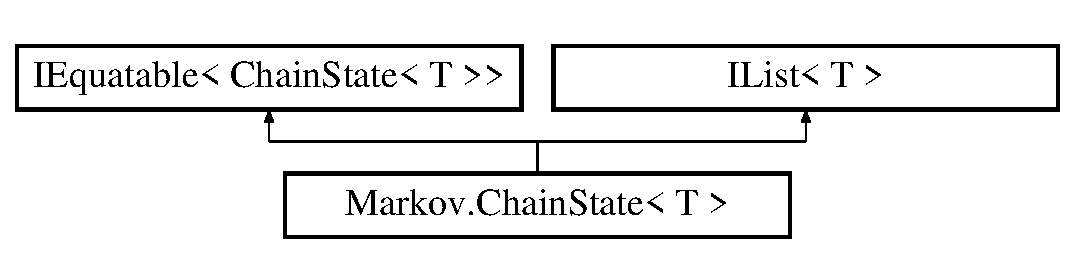
\includegraphics[height=2.000000cm]{class_markov_1_1_chain_state}
\end{center}
\end{figure}
\subsection*{Public Member Functions}
\begin{DoxyCompactItemize}
\item 
\mbox{\hyperlink{class_markov_1_1_chain_state_a350f2699a1eb55d8b041ff394c6ae3d4}{Chain\+State}} (I\+Enumerable$<$ T $>$ items)
\begin{DoxyCompactList}\small\item\em Initializes a new instance of the \mbox{\hyperlink{class_markov_1_1_chain_state_a350f2699a1eb55d8b041ff394c6ae3d4}{Chain\+State$<$\+T$>$}} class with the specified items. \end{DoxyCompactList}\item 
\mbox{\hyperlink{class_markov_1_1_chain_state_a69f3f9f56c55b4e31297d0c894c847a4}{Chain\+State}} (params T\mbox{[}$\,$\mbox{]} items)
\begin{DoxyCompactList}\small\item\em Initializes a new instance of the \mbox{\hyperlink{class_markov_1_1_chain_state_a350f2699a1eb55d8b041ff394c6ae3d4}{Chain\+State$<$\+T$>$}} class with the specified items. \end{DoxyCompactList}\item 
void \mbox{\hyperlink{class_markov_1_1_chain_state_abbc65b63c2626b9c575c18afbfcce28b}{Add}} (T item)
\item 
void \mbox{\hyperlink{class_markov_1_1_chain_state_aed8735821f05d6cde49beeb9e6d8cbe3}{Clear}} ()
\item 
bool \mbox{\hyperlink{class_markov_1_1_chain_state_a648edb3b1f6b26637588cc412a2d665f}{Contains}} (T item)
\item 
void \mbox{\hyperlink{class_markov_1_1_chain_state_a5ed671961c6e7e5fde9810d3b812bbac}{Copy\+To}} (T\mbox{[}$\,$\mbox{]} array, int array\+Index)
\item 
override bool \mbox{\hyperlink{class_markov_1_1_chain_state_a7774a491a81fcf44fd7777f3d58e57e5}{Equals}} (object obj)
\item 
bool \mbox{\hyperlink{class_markov_1_1_chain_state_ae7f0298aa37790cf06f6daf63e879c29}{Equals}} (\mbox{\hyperlink{class_markov_1_1_chain_state}{Chain\+State}}$<$ T $>$ other)
\begin{DoxyCompactList}\small\item\em Indicates whether the current object is equal to another object of the same type. \end{DoxyCompactList}\item 
I\+Enumerator$<$ T $>$ \mbox{\hyperlink{class_markov_1_1_chain_state_a81c94c2203e25ac36ba1ddd178fc2b15}{Get\+Enumerator}} ()
\item 
override int \mbox{\hyperlink{class_markov_1_1_chain_state_aaadb2ec85a68a5c70f18b0d163230134}{Get\+Hash\+Code}} ()
\item 
int \mbox{\hyperlink{class_markov_1_1_chain_state_a2af30e4d2673359b79bfaa6a2de48bf9}{Index\+Of}} (T item)
\item 
void \mbox{\hyperlink{class_markov_1_1_chain_state_ad5efce337d44856d13229069afff0879}{Insert}} (int index, T item)
\item 
bool \mbox{\hyperlink{class_markov_1_1_chain_state_a14ba6dd48c8f96ae8c396779ac6fbbc3}{Remove}} (T item)
\item 
void \mbox{\hyperlink{class_markov_1_1_chain_state_af04b4b8af2b5de82f276a74087a1d500}{Remove\+At}} (int index)
\end{DoxyCompactItemize}
\subsection*{Static Public Member Functions}
\begin{DoxyCompactItemize}
\item 
static bool \mbox{\hyperlink{class_markov_1_1_chain_state_a6461dd479522fd7d95f2e86a166187f4}{operator!=}} (\mbox{\hyperlink{class_markov_1_1_chain_state}{Chain\+State}}$<$ T $>$ a, \mbox{\hyperlink{class_markov_1_1_chain_state}{Chain\+State}}$<$ T $>$ b)
\begin{DoxyCompactList}\small\item\em Determines whether two specified instances of \mbox{\hyperlink{class_markov_1_1_chain_state_a350f2699a1eb55d8b041ff394c6ae3d4}{Chain\+State$<$\+T$>$}} are not equal. \end{DoxyCompactList}\item 
static bool \mbox{\hyperlink{class_markov_1_1_chain_state_a89707d9945ed200acc226df512001169}{operator==}} (\mbox{\hyperlink{class_markov_1_1_chain_state}{Chain\+State}}$<$ T $>$ a, \mbox{\hyperlink{class_markov_1_1_chain_state}{Chain\+State}}$<$ T $>$ b)
\begin{DoxyCompactList}\small\item\em Determines whether two specified instances of \mbox{\hyperlink{class_markov_1_1_chain_state_a350f2699a1eb55d8b041ff394c6ae3d4}{Chain\+State$<$\+T$>$}} are equal. \end{DoxyCompactList}\end{DoxyCompactItemize}
\subsection*{Public Attributes}
\begin{DoxyCompactItemize}
\item 
int \mbox{\hyperlink{class_markov_1_1_chain_state_a514640cd4bfd2d2fae5162305dd13990}{Count}} =$>$ this.\+items.\+Length
\item 
bool \mbox{\hyperlink{class_markov_1_1_chain_state_af899470e8c30912c17125b8d365bde02}{Is\+Read\+Only}} =$>$ true
\end{DoxyCompactItemize}
\subsection*{Properties}
\begin{DoxyCompactItemize}
\item 
T \mbox{\hyperlink{class_markov_1_1_chain_state_ae06f12faf66236f004133d5cd08b22b4}{this\mbox{[}int index\mbox{]}}}\hspace{0.3cm}{\ttfamily  \mbox{[}get, set\mbox{]}}
\end{DoxyCompactItemize}


\subsection{Detailed Description}
Represents a state in a \mbox{\hyperlink{namespace_markov}{Markov}} chain. 


\begin{DoxyTemplParams}{Template Parameters}
{\em T} & The type of the constituent parts of each state in the \mbox{\hyperlink{namespace_markov}{Markov}} chain.\\
\hline
\end{DoxyTemplParams}


\subsection{Constructor \& Destructor Documentation}
\mbox{\Hypertarget{class_markov_1_1_chain_state_a350f2699a1eb55d8b041ff394c6ae3d4}\label{class_markov_1_1_chain_state_a350f2699a1eb55d8b041ff394c6ae3d4}} 
\index{Markov\+::\+Chain\+State@{Markov\+::\+Chain\+State}!Chain\+State@{Chain\+State}}
\index{Chain\+State@{Chain\+State}!Markov\+::\+Chain\+State@{Markov\+::\+Chain\+State}}
\subsubsection{\texorpdfstring{Chain\+State()}{ChainState()}\hspace{0.1cm}{\footnotesize\ttfamily [1/2]}}
{\footnotesize\ttfamily \mbox{\hyperlink{class_markov_1_1_chain_state}{Markov.\+Chain\+State}}$<$ T $>$.\mbox{\hyperlink{class_markov_1_1_chain_state}{Chain\+State}} (\begin{DoxyParamCaption}\item[{I\+Enumerable$<$ T $>$}]{items }\end{DoxyParamCaption})}



Initializes a new instance of the \mbox{\hyperlink{class_markov_1_1_chain_state_a350f2699a1eb55d8b041ff394c6ae3d4}{Chain\+State$<$\+T$>$}} class with the specified items. 


\begin{DoxyParams}{Parameters}
{\em items} & An I\+Enumerable$<$\+T$>$ of items to be copied as a single state.\\
\hline
\end{DoxyParams}
\mbox{\Hypertarget{class_markov_1_1_chain_state_a69f3f9f56c55b4e31297d0c894c847a4}\label{class_markov_1_1_chain_state_a69f3f9f56c55b4e31297d0c894c847a4}} 
\index{Markov\+::\+Chain\+State@{Markov\+::\+Chain\+State}!Chain\+State@{Chain\+State}}
\index{Chain\+State@{Chain\+State}!Markov\+::\+Chain\+State@{Markov\+::\+Chain\+State}}
\subsubsection{\texorpdfstring{Chain\+State()}{ChainState()}\hspace{0.1cm}{\footnotesize\ttfamily [2/2]}}
{\footnotesize\ttfamily \mbox{\hyperlink{class_markov_1_1_chain_state}{Markov.\+Chain\+State}}$<$ T $>$.\mbox{\hyperlink{class_markov_1_1_chain_state}{Chain\+State}} (\begin{DoxyParamCaption}\item[{params T \mbox{[}$\,$\mbox{]}}]{items }\end{DoxyParamCaption})}



Initializes a new instance of the \mbox{\hyperlink{class_markov_1_1_chain_state_a350f2699a1eb55d8b041ff394c6ae3d4}{Chain\+State$<$\+T$>$}} class with the specified items. 


\begin{DoxyParams}{Parameters}
{\em items} & An array of {\itshape T}  items to be copied as a single state.\\
\hline
\end{DoxyParams}


\subsection{Member Function Documentation}
\mbox{\Hypertarget{class_markov_1_1_chain_state_abbc65b63c2626b9c575c18afbfcce28b}\label{class_markov_1_1_chain_state_abbc65b63c2626b9c575c18afbfcce28b}} 
\index{Markov\+::\+Chain\+State@{Markov\+::\+Chain\+State}!Add@{Add}}
\index{Add@{Add}!Markov\+::\+Chain\+State@{Markov\+::\+Chain\+State}}
\subsubsection{\texorpdfstring{Add()}{Add()}}
{\footnotesize\ttfamily void \mbox{\hyperlink{class_markov_1_1_chain_state}{Markov.\+Chain\+State}}$<$ T $>$.Add (\begin{DoxyParamCaption}\item[{T}]{item }\end{DoxyParamCaption})}





\mbox{\Hypertarget{class_markov_1_1_chain_state_aed8735821f05d6cde49beeb9e6d8cbe3}\label{class_markov_1_1_chain_state_aed8735821f05d6cde49beeb9e6d8cbe3}} 
\index{Markov\+::\+Chain\+State@{Markov\+::\+Chain\+State}!Clear@{Clear}}
\index{Clear@{Clear}!Markov\+::\+Chain\+State@{Markov\+::\+Chain\+State}}
\subsubsection{\texorpdfstring{Clear()}{Clear()}}
{\footnotesize\ttfamily void \mbox{\hyperlink{class_markov_1_1_chain_state}{Markov.\+Chain\+State}}$<$ T $>$.Clear (\begin{DoxyParamCaption}{ }\end{DoxyParamCaption})}





\mbox{\Hypertarget{class_markov_1_1_chain_state_a648edb3b1f6b26637588cc412a2d665f}\label{class_markov_1_1_chain_state_a648edb3b1f6b26637588cc412a2d665f}} 
\index{Markov\+::\+Chain\+State@{Markov\+::\+Chain\+State}!Contains@{Contains}}
\index{Contains@{Contains}!Markov\+::\+Chain\+State@{Markov\+::\+Chain\+State}}
\subsubsection{\texorpdfstring{Contains()}{Contains()}}
{\footnotesize\ttfamily bool \mbox{\hyperlink{class_markov_1_1_chain_state}{Markov.\+Chain\+State}}$<$ T $>$.Contains (\begin{DoxyParamCaption}\item[{T}]{item }\end{DoxyParamCaption})}





\mbox{\Hypertarget{class_markov_1_1_chain_state_a5ed671961c6e7e5fde9810d3b812bbac}\label{class_markov_1_1_chain_state_a5ed671961c6e7e5fde9810d3b812bbac}} 
\index{Markov\+::\+Chain\+State@{Markov\+::\+Chain\+State}!Copy\+To@{Copy\+To}}
\index{Copy\+To@{Copy\+To}!Markov\+::\+Chain\+State@{Markov\+::\+Chain\+State}}
\subsubsection{\texorpdfstring{Copy\+To()}{CopyTo()}}
{\footnotesize\ttfamily void \mbox{\hyperlink{class_markov_1_1_chain_state}{Markov.\+Chain\+State}}$<$ T $>$.Copy\+To (\begin{DoxyParamCaption}\item[{T \mbox{[}$\,$\mbox{]}}]{array,  }\item[{int}]{array\+Index }\end{DoxyParamCaption})}





\mbox{\Hypertarget{class_markov_1_1_chain_state_a7774a491a81fcf44fd7777f3d58e57e5}\label{class_markov_1_1_chain_state_a7774a491a81fcf44fd7777f3d58e57e5}} 
\index{Markov\+::\+Chain\+State@{Markov\+::\+Chain\+State}!Equals@{Equals}}
\index{Equals@{Equals}!Markov\+::\+Chain\+State@{Markov\+::\+Chain\+State}}
\subsubsection{\texorpdfstring{Equals()}{Equals()}\hspace{0.1cm}{\footnotesize\ttfamily [1/2]}}
{\footnotesize\ttfamily override bool \mbox{\hyperlink{class_markov_1_1_chain_state}{Markov.\+Chain\+State}}$<$ T $>$.Equals (\begin{DoxyParamCaption}\item[{object}]{obj }\end{DoxyParamCaption})}





\mbox{\Hypertarget{class_markov_1_1_chain_state_ae7f0298aa37790cf06f6daf63e879c29}\label{class_markov_1_1_chain_state_ae7f0298aa37790cf06f6daf63e879c29}} 
\index{Markov\+::\+Chain\+State@{Markov\+::\+Chain\+State}!Equals@{Equals}}
\index{Equals@{Equals}!Markov\+::\+Chain\+State@{Markov\+::\+Chain\+State}}
\subsubsection{\texorpdfstring{Equals()}{Equals()}\hspace{0.1cm}{\footnotesize\ttfamily [2/2]}}
{\footnotesize\ttfamily bool \mbox{\hyperlink{class_markov_1_1_chain_state}{Markov.\+Chain\+State}}$<$ T $>$.Equals (\begin{DoxyParamCaption}\item[{\mbox{\hyperlink{class_markov_1_1_chain_state}{Chain\+State}}$<$ T $>$}]{other }\end{DoxyParamCaption})}



Indicates whether the current object is equal to another object of the same type. 


\begin{DoxyParams}{Parameters}
{\em other} & An object to compare with this object.\\
\hline
\end{DoxyParams}
\begin{DoxyReturn}{Returns}
true if the current object is equal to the {\itshape other}  parameter; otherwise, false.
\end{DoxyReturn}
\mbox{\Hypertarget{class_markov_1_1_chain_state_a81c94c2203e25ac36ba1ddd178fc2b15}\label{class_markov_1_1_chain_state_a81c94c2203e25ac36ba1ddd178fc2b15}} 
\index{Markov\+::\+Chain\+State@{Markov\+::\+Chain\+State}!Get\+Enumerator@{Get\+Enumerator}}
\index{Get\+Enumerator@{Get\+Enumerator}!Markov\+::\+Chain\+State@{Markov\+::\+Chain\+State}}
\subsubsection{\texorpdfstring{Get\+Enumerator()}{GetEnumerator()}}
{\footnotesize\ttfamily I\+Enumerator$<$T$>$ \mbox{\hyperlink{class_markov_1_1_chain_state}{Markov.\+Chain\+State}}$<$ T $>$.Get\+Enumerator (\begin{DoxyParamCaption}{ }\end{DoxyParamCaption})}





\mbox{\Hypertarget{class_markov_1_1_chain_state_aaadb2ec85a68a5c70f18b0d163230134}\label{class_markov_1_1_chain_state_aaadb2ec85a68a5c70f18b0d163230134}} 
\index{Markov\+::\+Chain\+State@{Markov\+::\+Chain\+State}!Get\+Hash\+Code@{Get\+Hash\+Code}}
\index{Get\+Hash\+Code@{Get\+Hash\+Code}!Markov\+::\+Chain\+State@{Markov\+::\+Chain\+State}}
\subsubsection{\texorpdfstring{Get\+Hash\+Code()}{GetHashCode()}}
{\footnotesize\ttfamily override int \mbox{\hyperlink{class_markov_1_1_chain_state}{Markov.\+Chain\+State}}$<$ T $>$.Get\+Hash\+Code (\begin{DoxyParamCaption}{ }\end{DoxyParamCaption})}





\mbox{\Hypertarget{class_markov_1_1_chain_state_a2af30e4d2673359b79bfaa6a2de48bf9}\label{class_markov_1_1_chain_state_a2af30e4d2673359b79bfaa6a2de48bf9}} 
\index{Markov\+::\+Chain\+State@{Markov\+::\+Chain\+State}!Index\+Of@{Index\+Of}}
\index{Index\+Of@{Index\+Of}!Markov\+::\+Chain\+State@{Markov\+::\+Chain\+State}}
\subsubsection{\texorpdfstring{Index\+Of()}{IndexOf()}}
{\footnotesize\ttfamily int \mbox{\hyperlink{class_markov_1_1_chain_state}{Markov.\+Chain\+State}}$<$ T $>$.Index\+Of (\begin{DoxyParamCaption}\item[{T}]{item }\end{DoxyParamCaption})}





\mbox{\Hypertarget{class_markov_1_1_chain_state_ad5efce337d44856d13229069afff0879}\label{class_markov_1_1_chain_state_ad5efce337d44856d13229069afff0879}} 
\index{Markov\+::\+Chain\+State@{Markov\+::\+Chain\+State}!Insert@{Insert}}
\index{Insert@{Insert}!Markov\+::\+Chain\+State@{Markov\+::\+Chain\+State}}
\subsubsection{\texorpdfstring{Insert()}{Insert()}}
{\footnotesize\ttfamily void \mbox{\hyperlink{class_markov_1_1_chain_state}{Markov.\+Chain\+State}}$<$ T $>$.Insert (\begin{DoxyParamCaption}\item[{int}]{index,  }\item[{T}]{item }\end{DoxyParamCaption})}





\mbox{\Hypertarget{class_markov_1_1_chain_state_a6461dd479522fd7d95f2e86a166187f4}\label{class_markov_1_1_chain_state_a6461dd479522fd7d95f2e86a166187f4}} 
\index{Markov\+::\+Chain\+State@{Markov\+::\+Chain\+State}!operator"!=@{operator"!=}}
\index{operator"!=@{operator"!=}!Markov\+::\+Chain\+State@{Markov\+::\+Chain\+State}}
\subsubsection{\texorpdfstring{operator"!=()}{operator!=()}}
{\footnotesize\ttfamily static bool \mbox{\hyperlink{class_markov_1_1_chain_state}{Markov.\+Chain\+State}}$<$ T $>$.operator!= (\begin{DoxyParamCaption}\item[{\mbox{\hyperlink{class_markov_1_1_chain_state}{Chain\+State}}$<$ T $>$}]{a,  }\item[{\mbox{\hyperlink{class_markov_1_1_chain_state}{Chain\+State}}$<$ T $>$}]{b }\end{DoxyParamCaption})\hspace{0.3cm}{\ttfamily [static]}}



Determines whether two specified instances of \mbox{\hyperlink{class_markov_1_1_chain_state_a350f2699a1eb55d8b041ff394c6ae3d4}{Chain\+State$<$\+T$>$}} are not equal. 


\begin{DoxyParams}{Parameters}
{\em a} & The first \mbox{\hyperlink{class_markov_1_1_chain_state_a350f2699a1eb55d8b041ff394c6ae3d4}{Chain\+State$<$\+T$>$}} to compare.\\
\hline
{\em b} & The second \mbox{\hyperlink{class_markov_1_1_chain_state_a350f2699a1eb55d8b041ff394c6ae3d4}{Chain\+State$<$\+T$>$}} to compare.\\
\hline
\end{DoxyParams}
\begin{DoxyReturn}{Returns}
true if {\itshape a}  and {\itshape b}  do not represent the same state; otherwise, false.
\end{DoxyReturn}
\mbox{\Hypertarget{class_markov_1_1_chain_state_a89707d9945ed200acc226df512001169}\label{class_markov_1_1_chain_state_a89707d9945ed200acc226df512001169}} 
\index{Markov\+::\+Chain\+State@{Markov\+::\+Chain\+State}!operator==@{operator==}}
\index{operator==@{operator==}!Markov\+::\+Chain\+State@{Markov\+::\+Chain\+State}}
\subsubsection{\texorpdfstring{operator==()}{operator==()}}
{\footnotesize\ttfamily static bool \mbox{\hyperlink{class_markov_1_1_chain_state}{Markov.\+Chain\+State}}$<$ T $>$.operator== (\begin{DoxyParamCaption}\item[{\mbox{\hyperlink{class_markov_1_1_chain_state}{Chain\+State}}$<$ T $>$}]{a,  }\item[{\mbox{\hyperlink{class_markov_1_1_chain_state}{Chain\+State}}$<$ T $>$}]{b }\end{DoxyParamCaption})\hspace{0.3cm}{\ttfamily [static]}}



Determines whether two specified instances of \mbox{\hyperlink{class_markov_1_1_chain_state_a350f2699a1eb55d8b041ff394c6ae3d4}{Chain\+State$<$\+T$>$}} are equal. 


\begin{DoxyParams}{Parameters}
{\em a} & The first \mbox{\hyperlink{class_markov_1_1_chain_state_a350f2699a1eb55d8b041ff394c6ae3d4}{Chain\+State$<$\+T$>$}} to compare.\\
\hline
{\em b} & The second \mbox{\hyperlink{class_markov_1_1_chain_state_a350f2699a1eb55d8b041ff394c6ae3d4}{Chain\+State$<$\+T$>$}} to compare.\\
\hline
\end{DoxyParams}
\begin{DoxyReturn}{Returns}
true if {\itshape a}  and {\itshape b}  represent the same state; otherwise, false.
\end{DoxyReturn}
\mbox{\Hypertarget{class_markov_1_1_chain_state_a14ba6dd48c8f96ae8c396779ac6fbbc3}\label{class_markov_1_1_chain_state_a14ba6dd48c8f96ae8c396779ac6fbbc3}} 
\index{Markov\+::\+Chain\+State@{Markov\+::\+Chain\+State}!Remove@{Remove}}
\index{Remove@{Remove}!Markov\+::\+Chain\+State@{Markov\+::\+Chain\+State}}
\subsubsection{\texorpdfstring{Remove()}{Remove()}}
{\footnotesize\ttfamily bool \mbox{\hyperlink{class_markov_1_1_chain_state}{Markov.\+Chain\+State}}$<$ T $>$.Remove (\begin{DoxyParamCaption}\item[{T}]{item }\end{DoxyParamCaption})}





\mbox{\Hypertarget{class_markov_1_1_chain_state_af04b4b8af2b5de82f276a74087a1d500}\label{class_markov_1_1_chain_state_af04b4b8af2b5de82f276a74087a1d500}} 
\index{Markov\+::\+Chain\+State@{Markov\+::\+Chain\+State}!Remove\+At@{Remove\+At}}
\index{Remove\+At@{Remove\+At}!Markov\+::\+Chain\+State@{Markov\+::\+Chain\+State}}
\subsubsection{\texorpdfstring{Remove\+At()}{RemoveAt()}}
{\footnotesize\ttfamily void \mbox{\hyperlink{class_markov_1_1_chain_state}{Markov.\+Chain\+State}}$<$ T $>$.Remove\+At (\begin{DoxyParamCaption}\item[{int}]{index }\end{DoxyParamCaption})}







\subsection{Member Data Documentation}
\mbox{\Hypertarget{class_markov_1_1_chain_state_a514640cd4bfd2d2fae5162305dd13990}\label{class_markov_1_1_chain_state_a514640cd4bfd2d2fae5162305dd13990}} 
\index{Markov\+::\+Chain\+State@{Markov\+::\+Chain\+State}!Count@{Count}}
\index{Count@{Count}!Markov\+::\+Chain\+State@{Markov\+::\+Chain\+State}}
\subsubsection{\texorpdfstring{Count}{Count}}
{\footnotesize\ttfamily int \mbox{\hyperlink{class_markov_1_1_chain_state}{Markov.\+Chain\+State}}$<$ T $>$.Count =$>$ this.\+items.\+Length}





\mbox{\Hypertarget{class_markov_1_1_chain_state_af899470e8c30912c17125b8d365bde02}\label{class_markov_1_1_chain_state_af899470e8c30912c17125b8d365bde02}} 
\index{Markov\+::\+Chain\+State@{Markov\+::\+Chain\+State}!Is\+Read\+Only@{Is\+Read\+Only}}
\index{Is\+Read\+Only@{Is\+Read\+Only}!Markov\+::\+Chain\+State@{Markov\+::\+Chain\+State}}
\subsubsection{\texorpdfstring{Is\+Read\+Only}{IsReadOnly}}
{\footnotesize\ttfamily bool \mbox{\hyperlink{class_markov_1_1_chain_state}{Markov.\+Chain\+State}}$<$ T $>$.Is\+Read\+Only =$>$ true}







\subsection{Property Documentation}
\mbox{\Hypertarget{class_markov_1_1_chain_state_ae06f12faf66236f004133d5cd08b22b4}\label{class_markov_1_1_chain_state_ae06f12faf66236f004133d5cd08b22b4}} 
\index{Markov\+::\+Chain\+State@{Markov\+::\+Chain\+State}!this\mbox{[}int index\mbox{]}@{this[int index]}}
\index{this\mbox{[}int index\mbox{]}@{this[int index]}!Markov\+::\+Chain\+State@{Markov\+::\+Chain\+State}}
\subsubsection{\texorpdfstring{this[int index]}{this[int index]}}
{\footnotesize\ttfamily T \mbox{\hyperlink{class_markov_1_1_chain_state}{Markov.\+Chain\+State}}$<$ T $>$.this\mbox{[}int index\mbox{]}\hspace{0.3cm}{\ttfamily [get]}, {\ttfamily [set]}}







The documentation for this class was generated from the following file\+:\begin{DoxyCompactItemize}
\item 
D\+:/\+Jacob\+\_\+\+D/\+Documents/\+C\+O\+M\+P 8045 Game 2 backup/\+C\+O\+M\+P 8045 Game 2/\+Out of Assets-\/ofmarkov-\/master/markov-\/master/\+Markov/\mbox{\hyperlink{_chain_state_8cs}{Chain\+State.\+cs}}\end{DoxyCompactItemize}

\hypertarget{class_markov_1_1_tests_1_1_chain_state_tests}{}\section{Markov.\+Tests.\+Chain\+State\+Tests Class Reference}
\label{class_markov_1_1_tests_1_1_chain_state_tests}\index{Markov.\+Tests.\+Chain\+State\+Tests@{Markov.\+Tests.\+Chain\+State\+Tests}}
\subsection*{Public Member Functions}
\begin{DoxyCompactItemize}
\item 
void \mbox{\hyperlink{class_markov_1_1_tests_1_1_chain_state_tests_a1732c1d9f5264c4b3a4f7db62c382887}{Ctor\+\_\+\+With\+Null\+Array\+\_\+\+Throws\+Argument\+Null\+Exception}} ()
\item 
void \mbox{\hyperlink{class_markov_1_1_tests_1_1_chain_state_tests_a8df3344f8b729836e3906feee2ed6e0c}{Ctor\+\_\+\+With\+Null\+Enumerable\+\_\+\+Throws\+Argument\+Null\+Exception}} ()
\item 
void \mbox{\hyperlink{class_markov_1_1_tests_1_1_chain_state_tests_a6266a5a184b0027b239970f1bd4d3cd9}{Equals\+\_\+\+With\+Different\+Values\+\_\+\+Returns\+False}} (string value1, string value2)
\item 
void \mbox{\hyperlink{class_markov_1_1_tests_1_1_chain_state_tests_a2af281c58c6143a94872ab96e3c89628}{Equals\+\_\+\+With\+Null\+Reference\+\_\+\+Returns\+False}} (string value)
\item 
void \mbox{\hyperlink{class_markov_1_1_tests_1_1_chain_state_tests_a49715a98e44f2af604c8c89a17485604}{Equals\+\_\+\+With\+The\+Same\+Reference\+\_\+\+Returns\+True}} (string value)
\item 
void \mbox{\hyperlink{class_markov_1_1_tests_1_1_chain_state_tests_a7888494e8a911654f08738fa342c5bab}{Equals\+\_\+\+With\+The\+Same\+Value\+\_\+\+Returns\+True}} (string value)
\item 
void \mbox{\hyperlink{class_markov_1_1_tests_1_1_chain_state_tests_a2f32a420320db3b20a1b3f844c80703f}{Op\+Equality\+\_\+\+With\+Different\+Values\+\_\+\+Returns\+False}} (string value1, string value2)
\item 
void \mbox{\hyperlink{class_markov_1_1_tests_1_1_chain_state_tests_ab49265be64b847b6ff8fdca707df4726}{Op\+Equality\+\_\+\+With\+Null\+Reference\+\_\+\+Returns\+False}} (string value)
\item 
void \mbox{\hyperlink{class_markov_1_1_tests_1_1_chain_state_tests_afb7e6cbcf0b528e8323a62c39ef9702a}{Op\+Equality\+\_\+\+With\+The\+Same\+Reference\+\_\+\+Returns\+True}} (string value)
\item 
void \mbox{\hyperlink{class_markov_1_1_tests_1_1_chain_state_tests_af5c431448228c72446da26c4b43f09bc}{Op\+Equality\+\_\+\+With\+The\+Same\+Value\+\_\+\+Returns\+True}} (string value)
\item 
void \mbox{\hyperlink{class_markov_1_1_tests_1_1_chain_state_tests_a2206cf4056184bee3f3a228b9f6da5e7}{Op\+Inequality\+\_\+\+With\+Different\+Values\+\_\+\+Returns\+True}} (string value1, string value2)
\item 
void \mbox{\hyperlink{class_markov_1_1_tests_1_1_chain_state_tests_a6789f7656ecaee08a77399ba14aa9f72}{Op\+Inequality\+\_\+\+With\+Null\+Reference\+\_\+\+Returns\+True}} (string value)
\item 
void \mbox{\hyperlink{class_markov_1_1_tests_1_1_chain_state_tests_a8fc9b1913bd953585a0822bea1ecad17}{Op\+Inequality\+\_\+\+With\+The\+Same\+Reference\+\_\+\+Returns\+False}} (string value)
\item 
void \mbox{\hyperlink{class_markov_1_1_tests_1_1_chain_state_tests_a5edd5e8df76165cd14cb238dc6d80459}{Op\+Inequality\+\_\+\+With\+The\+Same\+Value\+\_\+\+Returns\+False}} (string value)
\end{DoxyCompactItemize}
\subsection*{Static Public Attributes}
\begin{DoxyCompactItemize}
\item 
static string \mbox{[}$\,$\mbox{]} \mbox{\hyperlink{class_markov_1_1_tests_1_1_chain_state_tests_ab07b0e6dcc3273b5cd6321278394e79f}{Samples}}
\item 
static object \mbox{[}$\,$\mbox{]}\mbox{[}$\,$\mbox{]} \mbox{\hyperlink{class_markov_1_1_tests_1_1_chain_state_tests_a6f995526349802f9aeb21d1f754727c4}{Value\+Pairs}}
\item 
static object \mbox{[}$\,$\mbox{]}\mbox{[}$\,$\mbox{]} \mbox{\hyperlink{class_markov_1_1_tests_1_1_chain_state_tests_a057932abae5917bee396f427da7c8262}{Values}}
\end{DoxyCompactItemize}


\subsection{Member Function Documentation}
\mbox{\Hypertarget{class_markov_1_1_tests_1_1_chain_state_tests_a1732c1d9f5264c4b3a4f7db62c382887}\label{class_markov_1_1_tests_1_1_chain_state_tests_a1732c1d9f5264c4b3a4f7db62c382887}} 
\index{Markov\+::\+Tests\+::\+Chain\+State\+Tests@{Markov\+::\+Tests\+::\+Chain\+State\+Tests}!Ctor\+\_\+\+With\+Null\+Array\+\_\+\+Throws\+Argument\+Null\+Exception@{Ctor\+\_\+\+With\+Null\+Array\+\_\+\+Throws\+Argument\+Null\+Exception}}
\index{Ctor\+\_\+\+With\+Null\+Array\+\_\+\+Throws\+Argument\+Null\+Exception@{Ctor\+\_\+\+With\+Null\+Array\+\_\+\+Throws\+Argument\+Null\+Exception}!Markov\+::\+Tests\+::\+Chain\+State\+Tests@{Markov\+::\+Tests\+::\+Chain\+State\+Tests}}
\subsubsection{\texorpdfstring{Ctor\+\_\+\+With\+Null\+Array\+\_\+\+Throws\+Argument\+Null\+Exception()}{Ctor\_WithNullArray\_ThrowsArgumentNullException()}}
{\footnotesize\ttfamily void Markov.\+Tests.\+Chain\+State\+Tests.\+Ctor\+\_\+\+With\+Null\+Array\+\_\+\+Throws\+Argument\+Null\+Exception (\begin{DoxyParamCaption}{ }\end{DoxyParamCaption})}

\mbox{\Hypertarget{class_markov_1_1_tests_1_1_chain_state_tests_a8df3344f8b729836e3906feee2ed6e0c}\label{class_markov_1_1_tests_1_1_chain_state_tests_a8df3344f8b729836e3906feee2ed6e0c}} 
\index{Markov\+::\+Tests\+::\+Chain\+State\+Tests@{Markov\+::\+Tests\+::\+Chain\+State\+Tests}!Ctor\+\_\+\+With\+Null\+Enumerable\+\_\+\+Throws\+Argument\+Null\+Exception@{Ctor\+\_\+\+With\+Null\+Enumerable\+\_\+\+Throws\+Argument\+Null\+Exception}}
\index{Ctor\+\_\+\+With\+Null\+Enumerable\+\_\+\+Throws\+Argument\+Null\+Exception@{Ctor\+\_\+\+With\+Null\+Enumerable\+\_\+\+Throws\+Argument\+Null\+Exception}!Markov\+::\+Tests\+::\+Chain\+State\+Tests@{Markov\+::\+Tests\+::\+Chain\+State\+Tests}}
\subsubsection{\texorpdfstring{Ctor\+\_\+\+With\+Null\+Enumerable\+\_\+\+Throws\+Argument\+Null\+Exception()}{Ctor\_WithNullEnumerable\_ThrowsArgumentNullException()}}
{\footnotesize\ttfamily void Markov.\+Tests.\+Chain\+State\+Tests.\+Ctor\+\_\+\+With\+Null\+Enumerable\+\_\+\+Throws\+Argument\+Null\+Exception (\begin{DoxyParamCaption}{ }\end{DoxyParamCaption})}

\mbox{\Hypertarget{class_markov_1_1_tests_1_1_chain_state_tests_a6266a5a184b0027b239970f1bd4d3cd9}\label{class_markov_1_1_tests_1_1_chain_state_tests_a6266a5a184b0027b239970f1bd4d3cd9}} 
\index{Markov\+::\+Tests\+::\+Chain\+State\+Tests@{Markov\+::\+Tests\+::\+Chain\+State\+Tests}!Equals\+\_\+\+With\+Different\+Values\+\_\+\+Returns\+False@{Equals\+\_\+\+With\+Different\+Values\+\_\+\+Returns\+False}}
\index{Equals\+\_\+\+With\+Different\+Values\+\_\+\+Returns\+False@{Equals\+\_\+\+With\+Different\+Values\+\_\+\+Returns\+False}!Markov\+::\+Tests\+::\+Chain\+State\+Tests@{Markov\+::\+Tests\+::\+Chain\+State\+Tests}}
\subsubsection{\texorpdfstring{Equals\+\_\+\+With\+Different\+Values\+\_\+\+Returns\+False()}{Equals\_WithDifferentValues\_ReturnsFalse()}}
{\footnotesize\ttfamily void Markov.\+Tests.\+Chain\+State\+Tests.\+Equals\+\_\+\+With\+Different\+Values\+\_\+\+Returns\+False (\begin{DoxyParamCaption}\item[{string}]{value1,  }\item[{string}]{value2 }\end{DoxyParamCaption})}

\mbox{\Hypertarget{class_markov_1_1_tests_1_1_chain_state_tests_a2af281c58c6143a94872ab96e3c89628}\label{class_markov_1_1_tests_1_1_chain_state_tests_a2af281c58c6143a94872ab96e3c89628}} 
\index{Markov\+::\+Tests\+::\+Chain\+State\+Tests@{Markov\+::\+Tests\+::\+Chain\+State\+Tests}!Equals\+\_\+\+With\+Null\+Reference\+\_\+\+Returns\+False@{Equals\+\_\+\+With\+Null\+Reference\+\_\+\+Returns\+False}}
\index{Equals\+\_\+\+With\+Null\+Reference\+\_\+\+Returns\+False@{Equals\+\_\+\+With\+Null\+Reference\+\_\+\+Returns\+False}!Markov\+::\+Tests\+::\+Chain\+State\+Tests@{Markov\+::\+Tests\+::\+Chain\+State\+Tests}}
\subsubsection{\texorpdfstring{Equals\+\_\+\+With\+Null\+Reference\+\_\+\+Returns\+False()}{Equals\_WithNullReference\_ReturnsFalse()}}
{\footnotesize\ttfamily void Markov.\+Tests.\+Chain\+State\+Tests.\+Equals\+\_\+\+With\+Null\+Reference\+\_\+\+Returns\+False (\begin{DoxyParamCaption}\item[{string}]{value }\end{DoxyParamCaption})}

\mbox{\Hypertarget{class_markov_1_1_tests_1_1_chain_state_tests_a49715a98e44f2af604c8c89a17485604}\label{class_markov_1_1_tests_1_1_chain_state_tests_a49715a98e44f2af604c8c89a17485604}} 
\index{Markov\+::\+Tests\+::\+Chain\+State\+Tests@{Markov\+::\+Tests\+::\+Chain\+State\+Tests}!Equals\+\_\+\+With\+The\+Same\+Reference\+\_\+\+Returns\+True@{Equals\+\_\+\+With\+The\+Same\+Reference\+\_\+\+Returns\+True}}
\index{Equals\+\_\+\+With\+The\+Same\+Reference\+\_\+\+Returns\+True@{Equals\+\_\+\+With\+The\+Same\+Reference\+\_\+\+Returns\+True}!Markov\+::\+Tests\+::\+Chain\+State\+Tests@{Markov\+::\+Tests\+::\+Chain\+State\+Tests}}
\subsubsection{\texorpdfstring{Equals\+\_\+\+With\+The\+Same\+Reference\+\_\+\+Returns\+True()}{Equals\_WithTheSameReference\_ReturnsTrue()}}
{\footnotesize\ttfamily void Markov.\+Tests.\+Chain\+State\+Tests.\+Equals\+\_\+\+With\+The\+Same\+Reference\+\_\+\+Returns\+True (\begin{DoxyParamCaption}\item[{string}]{value }\end{DoxyParamCaption})}

\mbox{\Hypertarget{class_markov_1_1_tests_1_1_chain_state_tests_a7888494e8a911654f08738fa342c5bab}\label{class_markov_1_1_tests_1_1_chain_state_tests_a7888494e8a911654f08738fa342c5bab}} 
\index{Markov\+::\+Tests\+::\+Chain\+State\+Tests@{Markov\+::\+Tests\+::\+Chain\+State\+Tests}!Equals\+\_\+\+With\+The\+Same\+Value\+\_\+\+Returns\+True@{Equals\+\_\+\+With\+The\+Same\+Value\+\_\+\+Returns\+True}}
\index{Equals\+\_\+\+With\+The\+Same\+Value\+\_\+\+Returns\+True@{Equals\+\_\+\+With\+The\+Same\+Value\+\_\+\+Returns\+True}!Markov\+::\+Tests\+::\+Chain\+State\+Tests@{Markov\+::\+Tests\+::\+Chain\+State\+Tests}}
\subsubsection{\texorpdfstring{Equals\+\_\+\+With\+The\+Same\+Value\+\_\+\+Returns\+True()}{Equals\_WithTheSameValue\_ReturnsTrue()}}
{\footnotesize\ttfamily void Markov.\+Tests.\+Chain\+State\+Tests.\+Equals\+\_\+\+With\+The\+Same\+Value\+\_\+\+Returns\+True (\begin{DoxyParamCaption}\item[{string}]{value }\end{DoxyParamCaption})}

\mbox{\Hypertarget{class_markov_1_1_tests_1_1_chain_state_tests_a2f32a420320db3b20a1b3f844c80703f}\label{class_markov_1_1_tests_1_1_chain_state_tests_a2f32a420320db3b20a1b3f844c80703f}} 
\index{Markov\+::\+Tests\+::\+Chain\+State\+Tests@{Markov\+::\+Tests\+::\+Chain\+State\+Tests}!Op\+Equality\+\_\+\+With\+Different\+Values\+\_\+\+Returns\+False@{Op\+Equality\+\_\+\+With\+Different\+Values\+\_\+\+Returns\+False}}
\index{Op\+Equality\+\_\+\+With\+Different\+Values\+\_\+\+Returns\+False@{Op\+Equality\+\_\+\+With\+Different\+Values\+\_\+\+Returns\+False}!Markov\+::\+Tests\+::\+Chain\+State\+Tests@{Markov\+::\+Tests\+::\+Chain\+State\+Tests}}
\subsubsection{\texorpdfstring{Op\+Equality\+\_\+\+With\+Different\+Values\+\_\+\+Returns\+False()}{OpEquality\_WithDifferentValues\_ReturnsFalse()}}
{\footnotesize\ttfamily void Markov.\+Tests.\+Chain\+State\+Tests.\+Op\+Equality\+\_\+\+With\+Different\+Values\+\_\+\+Returns\+False (\begin{DoxyParamCaption}\item[{string}]{value1,  }\item[{string}]{value2 }\end{DoxyParamCaption})}

\mbox{\Hypertarget{class_markov_1_1_tests_1_1_chain_state_tests_ab49265be64b847b6ff8fdca707df4726}\label{class_markov_1_1_tests_1_1_chain_state_tests_ab49265be64b847b6ff8fdca707df4726}} 
\index{Markov\+::\+Tests\+::\+Chain\+State\+Tests@{Markov\+::\+Tests\+::\+Chain\+State\+Tests}!Op\+Equality\+\_\+\+With\+Null\+Reference\+\_\+\+Returns\+False@{Op\+Equality\+\_\+\+With\+Null\+Reference\+\_\+\+Returns\+False}}
\index{Op\+Equality\+\_\+\+With\+Null\+Reference\+\_\+\+Returns\+False@{Op\+Equality\+\_\+\+With\+Null\+Reference\+\_\+\+Returns\+False}!Markov\+::\+Tests\+::\+Chain\+State\+Tests@{Markov\+::\+Tests\+::\+Chain\+State\+Tests}}
\subsubsection{\texorpdfstring{Op\+Equality\+\_\+\+With\+Null\+Reference\+\_\+\+Returns\+False()}{OpEquality\_WithNullReference\_ReturnsFalse()}}
{\footnotesize\ttfamily void Markov.\+Tests.\+Chain\+State\+Tests.\+Op\+Equality\+\_\+\+With\+Null\+Reference\+\_\+\+Returns\+False (\begin{DoxyParamCaption}\item[{string}]{value }\end{DoxyParamCaption})}

\mbox{\Hypertarget{class_markov_1_1_tests_1_1_chain_state_tests_afb7e6cbcf0b528e8323a62c39ef9702a}\label{class_markov_1_1_tests_1_1_chain_state_tests_afb7e6cbcf0b528e8323a62c39ef9702a}} 
\index{Markov\+::\+Tests\+::\+Chain\+State\+Tests@{Markov\+::\+Tests\+::\+Chain\+State\+Tests}!Op\+Equality\+\_\+\+With\+The\+Same\+Reference\+\_\+\+Returns\+True@{Op\+Equality\+\_\+\+With\+The\+Same\+Reference\+\_\+\+Returns\+True}}
\index{Op\+Equality\+\_\+\+With\+The\+Same\+Reference\+\_\+\+Returns\+True@{Op\+Equality\+\_\+\+With\+The\+Same\+Reference\+\_\+\+Returns\+True}!Markov\+::\+Tests\+::\+Chain\+State\+Tests@{Markov\+::\+Tests\+::\+Chain\+State\+Tests}}
\subsubsection{\texorpdfstring{Op\+Equality\+\_\+\+With\+The\+Same\+Reference\+\_\+\+Returns\+True()}{OpEquality\_WithTheSameReference\_ReturnsTrue()}}
{\footnotesize\ttfamily void Markov.\+Tests.\+Chain\+State\+Tests.\+Op\+Equality\+\_\+\+With\+The\+Same\+Reference\+\_\+\+Returns\+True (\begin{DoxyParamCaption}\item[{string}]{value }\end{DoxyParamCaption})}

\mbox{\Hypertarget{class_markov_1_1_tests_1_1_chain_state_tests_af5c431448228c72446da26c4b43f09bc}\label{class_markov_1_1_tests_1_1_chain_state_tests_af5c431448228c72446da26c4b43f09bc}} 
\index{Markov\+::\+Tests\+::\+Chain\+State\+Tests@{Markov\+::\+Tests\+::\+Chain\+State\+Tests}!Op\+Equality\+\_\+\+With\+The\+Same\+Value\+\_\+\+Returns\+True@{Op\+Equality\+\_\+\+With\+The\+Same\+Value\+\_\+\+Returns\+True}}
\index{Op\+Equality\+\_\+\+With\+The\+Same\+Value\+\_\+\+Returns\+True@{Op\+Equality\+\_\+\+With\+The\+Same\+Value\+\_\+\+Returns\+True}!Markov\+::\+Tests\+::\+Chain\+State\+Tests@{Markov\+::\+Tests\+::\+Chain\+State\+Tests}}
\subsubsection{\texorpdfstring{Op\+Equality\+\_\+\+With\+The\+Same\+Value\+\_\+\+Returns\+True()}{OpEquality\_WithTheSameValue\_ReturnsTrue()}}
{\footnotesize\ttfamily void Markov.\+Tests.\+Chain\+State\+Tests.\+Op\+Equality\+\_\+\+With\+The\+Same\+Value\+\_\+\+Returns\+True (\begin{DoxyParamCaption}\item[{string}]{value }\end{DoxyParamCaption})}

\mbox{\Hypertarget{class_markov_1_1_tests_1_1_chain_state_tests_a2206cf4056184bee3f3a228b9f6da5e7}\label{class_markov_1_1_tests_1_1_chain_state_tests_a2206cf4056184bee3f3a228b9f6da5e7}} 
\index{Markov\+::\+Tests\+::\+Chain\+State\+Tests@{Markov\+::\+Tests\+::\+Chain\+State\+Tests}!Op\+Inequality\+\_\+\+With\+Different\+Values\+\_\+\+Returns\+True@{Op\+Inequality\+\_\+\+With\+Different\+Values\+\_\+\+Returns\+True}}
\index{Op\+Inequality\+\_\+\+With\+Different\+Values\+\_\+\+Returns\+True@{Op\+Inequality\+\_\+\+With\+Different\+Values\+\_\+\+Returns\+True}!Markov\+::\+Tests\+::\+Chain\+State\+Tests@{Markov\+::\+Tests\+::\+Chain\+State\+Tests}}
\subsubsection{\texorpdfstring{Op\+Inequality\+\_\+\+With\+Different\+Values\+\_\+\+Returns\+True()}{OpInequality\_WithDifferentValues\_ReturnsTrue()}}
{\footnotesize\ttfamily void Markov.\+Tests.\+Chain\+State\+Tests.\+Op\+Inequality\+\_\+\+With\+Different\+Values\+\_\+\+Returns\+True (\begin{DoxyParamCaption}\item[{string}]{value1,  }\item[{string}]{value2 }\end{DoxyParamCaption})}

\mbox{\Hypertarget{class_markov_1_1_tests_1_1_chain_state_tests_a6789f7656ecaee08a77399ba14aa9f72}\label{class_markov_1_1_tests_1_1_chain_state_tests_a6789f7656ecaee08a77399ba14aa9f72}} 
\index{Markov\+::\+Tests\+::\+Chain\+State\+Tests@{Markov\+::\+Tests\+::\+Chain\+State\+Tests}!Op\+Inequality\+\_\+\+With\+Null\+Reference\+\_\+\+Returns\+True@{Op\+Inequality\+\_\+\+With\+Null\+Reference\+\_\+\+Returns\+True}}
\index{Op\+Inequality\+\_\+\+With\+Null\+Reference\+\_\+\+Returns\+True@{Op\+Inequality\+\_\+\+With\+Null\+Reference\+\_\+\+Returns\+True}!Markov\+::\+Tests\+::\+Chain\+State\+Tests@{Markov\+::\+Tests\+::\+Chain\+State\+Tests}}
\subsubsection{\texorpdfstring{Op\+Inequality\+\_\+\+With\+Null\+Reference\+\_\+\+Returns\+True()}{OpInequality\_WithNullReference\_ReturnsTrue()}}
{\footnotesize\ttfamily void Markov.\+Tests.\+Chain\+State\+Tests.\+Op\+Inequality\+\_\+\+With\+Null\+Reference\+\_\+\+Returns\+True (\begin{DoxyParamCaption}\item[{string}]{value }\end{DoxyParamCaption})}

\mbox{\Hypertarget{class_markov_1_1_tests_1_1_chain_state_tests_a8fc9b1913bd953585a0822bea1ecad17}\label{class_markov_1_1_tests_1_1_chain_state_tests_a8fc9b1913bd953585a0822bea1ecad17}} 
\index{Markov\+::\+Tests\+::\+Chain\+State\+Tests@{Markov\+::\+Tests\+::\+Chain\+State\+Tests}!Op\+Inequality\+\_\+\+With\+The\+Same\+Reference\+\_\+\+Returns\+False@{Op\+Inequality\+\_\+\+With\+The\+Same\+Reference\+\_\+\+Returns\+False}}
\index{Op\+Inequality\+\_\+\+With\+The\+Same\+Reference\+\_\+\+Returns\+False@{Op\+Inequality\+\_\+\+With\+The\+Same\+Reference\+\_\+\+Returns\+False}!Markov\+::\+Tests\+::\+Chain\+State\+Tests@{Markov\+::\+Tests\+::\+Chain\+State\+Tests}}
\subsubsection{\texorpdfstring{Op\+Inequality\+\_\+\+With\+The\+Same\+Reference\+\_\+\+Returns\+False()}{OpInequality\_WithTheSameReference\_ReturnsFalse()}}
{\footnotesize\ttfamily void Markov.\+Tests.\+Chain\+State\+Tests.\+Op\+Inequality\+\_\+\+With\+The\+Same\+Reference\+\_\+\+Returns\+False (\begin{DoxyParamCaption}\item[{string}]{value }\end{DoxyParamCaption})}

\mbox{\Hypertarget{class_markov_1_1_tests_1_1_chain_state_tests_a5edd5e8df76165cd14cb238dc6d80459}\label{class_markov_1_1_tests_1_1_chain_state_tests_a5edd5e8df76165cd14cb238dc6d80459}} 
\index{Markov\+::\+Tests\+::\+Chain\+State\+Tests@{Markov\+::\+Tests\+::\+Chain\+State\+Tests}!Op\+Inequality\+\_\+\+With\+The\+Same\+Value\+\_\+\+Returns\+False@{Op\+Inequality\+\_\+\+With\+The\+Same\+Value\+\_\+\+Returns\+False}}
\index{Op\+Inequality\+\_\+\+With\+The\+Same\+Value\+\_\+\+Returns\+False@{Op\+Inequality\+\_\+\+With\+The\+Same\+Value\+\_\+\+Returns\+False}!Markov\+::\+Tests\+::\+Chain\+State\+Tests@{Markov\+::\+Tests\+::\+Chain\+State\+Tests}}
\subsubsection{\texorpdfstring{Op\+Inequality\+\_\+\+With\+The\+Same\+Value\+\_\+\+Returns\+False()}{OpInequality\_WithTheSameValue\_ReturnsFalse()}}
{\footnotesize\ttfamily void Markov.\+Tests.\+Chain\+State\+Tests.\+Op\+Inequality\+\_\+\+With\+The\+Same\+Value\+\_\+\+Returns\+False (\begin{DoxyParamCaption}\item[{string}]{value }\end{DoxyParamCaption})}



\subsection{Member Data Documentation}
\mbox{\Hypertarget{class_markov_1_1_tests_1_1_chain_state_tests_ab07b0e6dcc3273b5cd6321278394e79f}\label{class_markov_1_1_tests_1_1_chain_state_tests_ab07b0e6dcc3273b5cd6321278394e79f}} 
\index{Markov\+::\+Tests\+::\+Chain\+State\+Tests@{Markov\+::\+Tests\+::\+Chain\+State\+Tests}!Samples@{Samples}}
\index{Samples@{Samples}!Markov\+::\+Tests\+::\+Chain\+State\+Tests@{Markov\+::\+Tests\+::\+Chain\+State\+Tests}}
\subsubsection{\texorpdfstring{Samples}{Samples}}
{\footnotesize\ttfamily string \mbox{[}$\,$\mbox{]} Markov.\+Tests.\+Chain\+State\+Tests.\+Samples\hspace{0.3cm}{\ttfamily [static]}}

{\bfseries Initial value\+:}
\begin{DoxyCode}
=> \textcolor{keyword}{new}[]
        \{
            \textcolor{stringliteral}{"a"},
            \textcolor{stringliteral}{"ab"},
            \textcolor{stringliteral}{"abc"},
            \textcolor{stringliteral}{"aaa"},
        \}
\end{DoxyCode}
\mbox{\Hypertarget{class_markov_1_1_tests_1_1_chain_state_tests_a6f995526349802f9aeb21d1f754727c4}\label{class_markov_1_1_tests_1_1_chain_state_tests_a6f995526349802f9aeb21d1f754727c4}} 
\index{Markov\+::\+Tests\+::\+Chain\+State\+Tests@{Markov\+::\+Tests\+::\+Chain\+State\+Tests}!Value\+Pairs@{Value\+Pairs}}
\index{Value\+Pairs@{Value\+Pairs}!Markov\+::\+Tests\+::\+Chain\+State\+Tests@{Markov\+::\+Tests\+::\+Chain\+State\+Tests}}
\subsubsection{\texorpdfstring{Value\+Pairs}{ValuePairs}}
{\footnotesize\ttfamily object \mbox{[}$\,$\mbox{]}\mbox{[}$\,$\mbox{]} Markov.\+Tests.\+Chain\+State\+Tests.\+Value\+Pairs\hspace{0.3cm}{\ttfamily [static]}}

{\bfseries Initial value\+:}
\begin{DoxyCode}
=>
            (from v1 in \mbox{\hyperlink{class_markov_1_1_tests_1_1_chain_state_tests_ab07b0e6dcc3273b5cd6321278394e79f}{Samples}}
             from v2 in \mbox{\hyperlink{class_markov_1_1_tests_1_1_chain_state_tests_ab07b0e6dcc3273b5cd6321278394e79f}{Samples}}
             where v1 != v2
             select \textcolor{keyword}{new}[] \{ v1, v2 \}).ToArray()
\end{DoxyCode}
\mbox{\Hypertarget{class_markov_1_1_tests_1_1_chain_state_tests_a057932abae5917bee396f427da7c8262}\label{class_markov_1_1_tests_1_1_chain_state_tests_a057932abae5917bee396f427da7c8262}} 
\index{Markov\+::\+Tests\+::\+Chain\+State\+Tests@{Markov\+::\+Tests\+::\+Chain\+State\+Tests}!Values@{Values}}
\index{Values@{Values}!Markov\+::\+Tests\+::\+Chain\+State\+Tests@{Markov\+::\+Tests\+::\+Chain\+State\+Tests}}
\subsubsection{\texorpdfstring{Values}{Values}}
{\footnotesize\ttfamily object \mbox{[}$\,$\mbox{]}\mbox{[}$\,$\mbox{]} Markov.\+Tests.\+Chain\+State\+Tests.\+Values\hspace{0.3cm}{\ttfamily [static]}}

{\bfseries Initial value\+:}
\begin{DoxyCode}
=>
            (from v in \mbox{\hyperlink{class_markov_1_1_tests_1_1_chain_state_tests_ab07b0e6dcc3273b5cd6321278394e79f}{Samples}}
             select \textcolor{keyword}{new}[] \{ v \}).ToArray()
\end{DoxyCode}


The documentation for this class was generated from the following file\+:\begin{DoxyCompactItemize}
\item 
D\+:/\+Jacob\+\_\+\+D/\+Documents/\+C\+O\+M\+P 8045 Game 2 backup/\+C\+O\+M\+P 8045 Game 2/\+Out of Assets-\/ofmarkov-\/master/markov-\/master/\+Markov.\+Tests/\mbox{\hyperlink{_chain_state_tests_8cs}{Chain\+State\+Tests.\+cs}}\end{DoxyCompactItemize}

\hypertarget{class_markov_1_1_markov_chain}{}\section{Markov.\+Markov\+Chain$<$ T $>$ Class Template Reference}
\label{class_markov_1_1_markov_chain}\index{Markov.\+Markov\+Chain$<$ T $>$@{Markov.\+Markov\+Chain$<$ T $>$}}


Builds and walks interconnected states based on a weighted probability.  


\subsection*{Public Member Functions}
\begin{DoxyCompactItemize}
\item 
\mbox{\hyperlink{class_markov_1_1_markov_chain_a9cb6d5ce158a936323be57ae55622086}{Markov\+Chain}} (int order)
\begin{DoxyCompactList}\small\item\em Initializes a new instance of the \mbox{\hyperlink{class_markov_1_1_markov_chain_a9cb6d5ce158a936323be57ae55622086}{Markov\+Chain$<$\+T$>$}} class. \end{DoxyCompactList}\item 
void \mbox{\hyperlink{class_markov_1_1_markov_chain_abbdb660ed58d7eed8266dabba4bc29a4}{Add}} (I\+Enumerable$<$ T $>$ items)
\begin{DoxyCompactList}\small\item\em Adds the items to the generator with a weight of one. \end{DoxyCompactList}\item 
void \mbox{\hyperlink{class_markov_1_1_markov_chain_a4c3ca6b8cea20daf5c86cb1f5996c08b}{Add}} (I\+Enumerable$<$ T $>$ items, int weight)
\begin{DoxyCompactList}\small\item\em Adds the items to the generator with the weight specified. \end{DoxyCompactList}\item 
void \mbox{\hyperlink{class_markov_1_1_markov_chain_a3de9dba327e1da281f2fb8b5b267b4bc}{Add}} (I\+Enumerable$<$ T $>$ previous, T item)
\begin{DoxyCompactList}\small\item\em Adds the item to the generator, with the specified items preceding it. \end{DoxyCompactList}\item 
void \mbox{\hyperlink{class_markov_1_1_markov_chain_a70cf0423ef0109be16558b0765ec834d}{Add}} (\mbox{\hyperlink{class_markov_1_1_chain_state}{Chain\+State}}$<$ T $>$ state, T next)
\begin{DoxyCompactList}\small\item\em Adds the item to the generator, with the specified state preceding it. \end{DoxyCompactList}\item 
void \mbox{\hyperlink{class_markov_1_1_markov_chain_a3462f45546eaa3fd7c9592ca022a9ac6}{Add}} (I\+Enumerable$<$ T $>$ previous, T item, int weight)
\begin{DoxyCompactList}\small\item\em Adds the item to the generator, with the specified items preceding it and the specified weight. \end{DoxyCompactList}\item 
void \mbox{\hyperlink{class_markov_1_1_markov_chain_acbed62418075266c64c6e63d50726192}{Add}} (\mbox{\hyperlink{class_markov_1_1_chain_state}{Chain\+State}}$<$ T $>$ state, T next, int weight)
\begin{DoxyCompactList}\small\item\em Adds the item to the generator, with the specified state preceding it and the specified weight. \end{DoxyCompactList}\item 
I\+Enumerable$<$ T $>$ \mbox{\hyperlink{class_markov_1_1_markov_chain_a2748fc7f6e411bbbef965f4eaf7e5276}{Chain}} ()
\begin{DoxyCompactList}\small\item\em Randomly walks the chain. \end{DoxyCompactList}\item 
I\+Enumerable$<$ T $>$ \mbox{\hyperlink{class_markov_1_1_markov_chain_a2a851d551132a3c0b986ffdc435d94fa}{Chain}} (I\+Enumerable$<$ T $>$ previous)
\begin{DoxyCompactList}\small\item\em Randomly walks the chain. \end{DoxyCompactList}\item 
I\+Enumerable$<$ T $>$ \mbox{\hyperlink{class_markov_1_1_markov_chain_a4abb9314bca458994acd685a9357e1a0}{Chain}} (int seed)
\begin{DoxyCompactList}\small\item\em Randomly walks the chain. \end{DoxyCompactList}\item 
I\+Enumerable$<$ T $>$ \mbox{\hyperlink{class_markov_1_1_markov_chain_a325079fed5b93f2207814fa44a8108da}{Chain}} (I\+Enumerable$<$ T $>$ previous, int seed)
\begin{DoxyCompactList}\small\item\em Randomly walks the chain. \end{DoxyCompactList}\item 
I\+Enumerable$<$ T $>$ \mbox{\hyperlink{class_markov_1_1_markov_chain_a5d82b8169c681429fe8705b83bcb381e}{Chain}} (Random rand)
\begin{DoxyCompactList}\small\item\em Randomly walks the chain. \end{DoxyCompactList}\item 
I\+Enumerable$<$ T $>$ \mbox{\hyperlink{class_markov_1_1_markov_chain_a380daf4363822c659489862de2154dc1}{Chain}} (I\+Enumerable$<$ T $>$ previous, Random rand)
\begin{DoxyCompactList}\small\item\em Randomly walks the chain. \end{DoxyCompactList}\item 
Dictionary$<$ T, int $>$ \mbox{\hyperlink{class_markov_1_1_markov_chain_a5c19f54cdeff94bd0041fad4ba4c7c9e}{Get\+Initial\+States}} ()
\begin{DoxyCompactList}\small\item\em Gets the items from the generator that follow from an empty state. \end{DoxyCompactList}\item 
Dictionary$<$ T, int $>$ \mbox{\hyperlink{class_markov_1_1_markov_chain_aa9bf95df2986fff7d75c0c8489a0eab5}{Get\+Next\+States}} (I\+Enumerable$<$ T $>$ previous)
\begin{DoxyCompactList}\small\item\em Gets the items from the generator that follow from the specified items preceding it. \end{DoxyCompactList}\item 
Dictionary$<$ T, int $>$ \mbox{\hyperlink{class_markov_1_1_markov_chain_a124133e485b50cae03d205b5fcffcdb1}{Get\+Next\+States}} (\mbox{\hyperlink{class_markov_1_1_chain_state}{Chain\+State}}$<$ T $>$ state)
\begin{DoxyCompactList}\small\item\em Gets the items from the generator that follow from the specified state preceding it. \end{DoxyCompactList}\item 
I\+Enumerable$<$ \mbox{\hyperlink{class_markov_1_1_chain_state}{Chain\+State}}$<$ T $>$ $>$ \mbox{\hyperlink{class_markov_1_1_markov_chain_a5875741ce2c4fb9cb3d2242cac166167}{Get\+States}} ()
\begin{DoxyCompactList}\small\item\em Gets all of the states that exist in the generator. \end{DoxyCompactList}\item 
int \mbox{\hyperlink{class_markov_1_1_markov_chain_a893aace9c71c5837682db3827a5a2426}{Get\+Terminal\+Weight}} (I\+Enumerable$<$ T $>$ previous)
\begin{DoxyCompactList}\small\item\em Gets the weight of termination following from the specified items. \end{DoxyCompactList}\item 
int \mbox{\hyperlink{class_markov_1_1_markov_chain_a51cbf6330b16387447e761749161b768}{Get\+Terminal\+Weight}} (\mbox{\hyperlink{class_markov_1_1_chain_state}{Chain\+State}}$<$ T $>$ state)
\begin{DoxyCompactList}\small\item\em Gets the weights of termination following from the specified state. \end{DoxyCompactList}\end{DoxyCompactItemize}


\subsection{Detailed Description}
Builds and walks interconnected states based on a weighted probability. 


\begin{DoxyTemplParams}{Template Parameters}
{\em T} & The type of the constituent parts of each state in the \mbox{\hyperlink{namespace_markov}{Markov}} chain.\\
\hline
\end{DoxyTemplParams}
\begin{Desc}
\item[Type Constraints]\begin{description}
\item[{\em T} : {\em I\+Equatable$<$T$>$}]\end{description}
\end{Desc}


\subsection{Constructor \& Destructor Documentation}
\mbox{\Hypertarget{class_markov_1_1_markov_chain_a9cb6d5ce158a936323be57ae55622086}\label{class_markov_1_1_markov_chain_a9cb6d5ce158a936323be57ae55622086}} 
\index{Markov\+::\+Markov\+Chain@{Markov\+::\+Markov\+Chain}!Markov\+Chain@{Markov\+Chain}}
\index{Markov\+Chain@{Markov\+Chain}!Markov\+::\+Markov\+Chain@{Markov\+::\+Markov\+Chain}}
\subsubsection{\texorpdfstring{Markov\+Chain()}{MarkovChain()}}
{\footnotesize\ttfamily \mbox{\hyperlink{class_markov_1_1_markov_chain}{Markov.\+Markov\+Chain}}$<$ T $>$.\mbox{\hyperlink{class_markov_1_1_markov_chain}{Markov\+Chain}} (\begin{DoxyParamCaption}\item[{int}]{order }\end{DoxyParamCaption})}



Initializes a new instance of the \mbox{\hyperlink{class_markov_1_1_markov_chain_a9cb6d5ce158a936323be57ae55622086}{Markov\+Chain$<$\+T$>$}} class. 


\begin{DoxyParams}{Parameters}
{\em order} & Indicates the desired order of the \mbox{\hyperlink{class_markov_1_1_markov_chain_a9cb6d5ce158a936323be57ae55622086}{Markov\+Chain$<$\+T$>$}}.\\
\hline
\end{DoxyParams}


The {\itshape order}  of a generator indicates the depth of its internal state. A generator with an order of 1 will choose items based on the previous item, a generator with an order of 2 will choose items based on the previous 2 items, and so on.

Zero is not classically a valid order value, but it is allowed here. Choosing a zero value has the effect that every state is equivalent to the starting state, and so items will be chosen based on their total frequency.

\subsection{Member Function Documentation}
\mbox{\Hypertarget{class_markov_1_1_markov_chain_abbdb660ed58d7eed8266dabba4bc29a4}\label{class_markov_1_1_markov_chain_abbdb660ed58d7eed8266dabba4bc29a4}} 
\index{Markov\+::\+Markov\+Chain@{Markov\+::\+Markov\+Chain}!Add@{Add}}
\index{Add@{Add}!Markov\+::\+Markov\+Chain@{Markov\+::\+Markov\+Chain}}
\subsubsection{\texorpdfstring{Add()}{Add()}\hspace{0.1cm}{\footnotesize\ttfamily [1/6]}}
{\footnotesize\ttfamily void \mbox{\hyperlink{class_markov_1_1_markov_chain}{Markov.\+Markov\+Chain}}$<$ T $>$.Add (\begin{DoxyParamCaption}\item[{I\+Enumerable$<$ T $>$}]{items }\end{DoxyParamCaption})}



Adds the items to the generator with a weight of one. 


\begin{DoxyParams}{Parameters}
{\em items} & The items to add to the generator.\\
\hline
\end{DoxyParams}
\mbox{\Hypertarget{class_markov_1_1_markov_chain_a4c3ca6b8cea20daf5c86cb1f5996c08b}\label{class_markov_1_1_markov_chain_a4c3ca6b8cea20daf5c86cb1f5996c08b}} 
\index{Markov\+::\+Markov\+Chain@{Markov\+::\+Markov\+Chain}!Add@{Add}}
\index{Add@{Add}!Markov\+::\+Markov\+Chain@{Markov\+::\+Markov\+Chain}}
\subsubsection{\texorpdfstring{Add()}{Add()}\hspace{0.1cm}{\footnotesize\ttfamily [2/6]}}
{\footnotesize\ttfamily void \mbox{\hyperlink{class_markov_1_1_markov_chain}{Markov.\+Markov\+Chain}}$<$ T $>$.Add (\begin{DoxyParamCaption}\item[{I\+Enumerable$<$ T $>$}]{items,  }\item[{int}]{weight }\end{DoxyParamCaption})}



Adds the items to the generator with the weight specified. 


\begin{DoxyParams}{Parameters}
{\em items} & The items to add to the generator.\\
\hline
{\em weight} & The weight at which to add the items.\\
\hline
\end{DoxyParams}
\mbox{\Hypertarget{class_markov_1_1_markov_chain_a3de9dba327e1da281f2fb8b5b267b4bc}\label{class_markov_1_1_markov_chain_a3de9dba327e1da281f2fb8b5b267b4bc}} 
\index{Markov\+::\+Markov\+Chain@{Markov\+::\+Markov\+Chain}!Add@{Add}}
\index{Add@{Add}!Markov\+::\+Markov\+Chain@{Markov\+::\+Markov\+Chain}}
\subsubsection{\texorpdfstring{Add()}{Add()}\hspace{0.1cm}{\footnotesize\ttfamily [3/6]}}
{\footnotesize\ttfamily void \mbox{\hyperlink{class_markov_1_1_markov_chain}{Markov.\+Markov\+Chain}}$<$ T $>$.Add (\begin{DoxyParamCaption}\item[{I\+Enumerable$<$ T $>$}]{previous,  }\item[{T}]{item }\end{DoxyParamCaption})}



Adds the item to the generator, with the specified items preceding it. 


\begin{DoxyParams}{Parameters}
{\em previous} & The items preceding the item.\\
\hline
{\em item} & The item to add.\\
\hline
\end{DoxyParams}


See \mbox{\hyperlink{class_markov_1_1_markov_chain_a3462f45546eaa3fd7c9592ca022a9ac6}{Markov\+Chain$<$\+T$>$.\+Add(\+I\+Enumerable$<$\+T$>$, T, int)}} for remarks. \mbox{\Hypertarget{class_markov_1_1_markov_chain_a70cf0423ef0109be16558b0765ec834d}\label{class_markov_1_1_markov_chain_a70cf0423ef0109be16558b0765ec834d}} 
\index{Markov\+::\+Markov\+Chain@{Markov\+::\+Markov\+Chain}!Add@{Add}}
\index{Add@{Add}!Markov\+::\+Markov\+Chain@{Markov\+::\+Markov\+Chain}}
\subsubsection{\texorpdfstring{Add()}{Add()}\hspace{0.1cm}{\footnotesize\ttfamily [4/6]}}
{\footnotesize\ttfamily void \mbox{\hyperlink{class_markov_1_1_markov_chain}{Markov.\+Markov\+Chain}}$<$ T $>$.Add (\begin{DoxyParamCaption}\item[{\mbox{\hyperlink{class_markov_1_1_chain_state}{Chain\+State}}$<$ T $>$}]{state,  }\item[{T}]{next }\end{DoxyParamCaption})}



Adds the item to the generator, with the specified state preceding it. 


\begin{DoxyParams}{Parameters}
{\em state} & The state preceding the item.\\
\hline
{\em next} & The item to add.\\
\hline
\end{DoxyParams}


See \mbox{\hyperlink{class_markov_1_1_markov_chain_acbed62418075266c64c6e63d50726192}{Markov\+Chain$<$\+T$>$.\+Add(\+Chain\+State$<$\+T$>$, T, int)}} for remarks. \mbox{\Hypertarget{class_markov_1_1_markov_chain_a3462f45546eaa3fd7c9592ca022a9ac6}\label{class_markov_1_1_markov_chain_a3462f45546eaa3fd7c9592ca022a9ac6}} 
\index{Markov\+::\+Markov\+Chain@{Markov\+::\+Markov\+Chain}!Add@{Add}}
\index{Add@{Add}!Markov\+::\+Markov\+Chain@{Markov\+::\+Markov\+Chain}}
\subsubsection{\texorpdfstring{Add()}{Add()}\hspace{0.1cm}{\footnotesize\ttfamily [5/6]}}
{\footnotesize\ttfamily void \mbox{\hyperlink{class_markov_1_1_markov_chain}{Markov.\+Markov\+Chain}}$<$ T $>$.Add (\begin{DoxyParamCaption}\item[{I\+Enumerable$<$ T $>$}]{previous,  }\item[{T}]{item,  }\item[{int}]{weight }\end{DoxyParamCaption})}



Adds the item to the generator, with the specified items preceding it and the specified weight. 


\begin{DoxyParams}{Parameters}
{\em previous} & The items preceding the item.\\
\hline
{\em item} & The item to add.\\
\hline
{\em weight} & The weight of the item to add.\\
\hline
\end{DoxyParams}


This method does not add all of the preceding states to the generator. Notably, the empty state is not added, unless the {\itshape previous}  parameter is empty. \mbox{\Hypertarget{class_markov_1_1_markov_chain_acbed62418075266c64c6e63d50726192}\label{class_markov_1_1_markov_chain_acbed62418075266c64c6e63d50726192}} 
\index{Markov\+::\+Markov\+Chain@{Markov\+::\+Markov\+Chain}!Add@{Add}}
\index{Add@{Add}!Markov\+::\+Markov\+Chain@{Markov\+::\+Markov\+Chain}}
\subsubsection{\texorpdfstring{Add()}{Add()}\hspace{0.1cm}{\footnotesize\ttfamily [6/6]}}
{\footnotesize\ttfamily void \mbox{\hyperlink{class_markov_1_1_markov_chain}{Markov.\+Markov\+Chain}}$<$ T $>$.Add (\begin{DoxyParamCaption}\item[{\mbox{\hyperlink{class_markov_1_1_chain_state}{Chain\+State}}$<$ T $>$}]{state,  }\item[{T}]{next,  }\item[{int}]{weight }\end{DoxyParamCaption})}



Adds the item to the generator, with the specified state preceding it and the specified weight. 


\begin{DoxyParams}{Parameters}
{\em state} & The state preceding the item.\\
\hline
{\em next} & The item to add.\\
\hline
{\em weight} & The weight of the item to add.\\
\hline
\end{DoxyParams}


This adds the state as-\/is. The state may not be reachable if, for example, the number of items in the state is greater than the order of the generator, or if the combination of items is not available in the other states of the generator.

A negative weight may be passed, which will have the impact of reducing the weight of the specified state transition. This can therefore be used to remove items from the generator. The resulting weight will never be allowed below zero. \mbox{\Hypertarget{class_markov_1_1_markov_chain_a2748fc7f6e411bbbef965f4eaf7e5276}\label{class_markov_1_1_markov_chain_a2748fc7f6e411bbbef965f4eaf7e5276}} 
\index{Markov\+::\+Markov\+Chain@{Markov\+::\+Markov\+Chain}!Chain@{Chain}}
\index{Chain@{Chain}!Markov\+::\+Markov\+Chain@{Markov\+::\+Markov\+Chain}}
\subsubsection{\texorpdfstring{Chain()}{Chain()}\hspace{0.1cm}{\footnotesize\ttfamily [1/6]}}
{\footnotesize\ttfamily I\+Enumerable$<$T$>$ \mbox{\hyperlink{class_markov_1_1_markov_chain}{Markov.\+Markov\+Chain}}$<$ T $>$.Chain (\begin{DoxyParamCaption}{ }\end{DoxyParamCaption})}



Randomly walks the chain. 

\begin{DoxyReturn}{Returns}
An I\+Enumerable$<$\+T$>$ of the items chosen.
\end{DoxyReturn}


Assumes an empty starting state.\mbox{\Hypertarget{class_markov_1_1_markov_chain_a2a851d551132a3c0b986ffdc435d94fa}\label{class_markov_1_1_markov_chain_a2a851d551132a3c0b986ffdc435d94fa}} 
\index{Markov\+::\+Markov\+Chain@{Markov\+::\+Markov\+Chain}!Chain@{Chain}}
\index{Chain@{Chain}!Markov\+::\+Markov\+Chain@{Markov\+::\+Markov\+Chain}}
\subsubsection{\texorpdfstring{Chain()}{Chain()}\hspace{0.1cm}{\footnotesize\ttfamily [2/6]}}
{\footnotesize\ttfamily I\+Enumerable$<$T$>$ \mbox{\hyperlink{class_markov_1_1_markov_chain}{Markov.\+Markov\+Chain}}$<$ T $>$.Chain (\begin{DoxyParamCaption}\item[{I\+Enumerable$<$ T $>$}]{previous }\end{DoxyParamCaption})}



Randomly walks the chain. 


\begin{DoxyParams}{Parameters}
{\em previous} & The items preceding the first item in the chain.\\
\hline
\end{DoxyParams}
\begin{DoxyReturn}{Returns}
An I\+Enumerable$<$\+T$>$ of the items chosen.
\end{DoxyReturn}
\mbox{\Hypertarget{class_markov_1_1_markov_chain_a4abb9314bca458994acd685a9357e1a0}\label{class_markov_1_1_markov_chain_a4abb9314bca458994acd685a9357e1a0}} 
\index{Markov\+::\+Markov\+Chain@{Markov\+::\+Markov\+Chain}!Chain@{Chain}}
\index{Chain@{Chain}!Markov\+::\+Markov\+Chain@{Markov\+::\+Markov\+Chain}}
\subsubsection{\texorpdfstring{Chain()}{Chain()}\hspace{0.1cm}{\footnotesize\ttfamily [3/6]}}
{\footnotesize\ttfamily I\+Enumerable$<$T$>$ \mbox{\hyperlink{class_markov_1_1_markov_chain}{Markov.\+Markov\+Chain}}$<$ T $>$.Chain (\begin{DoxyParamCaption}\item[{int}]{seed }\end{DoxyParamCaption})}



Randomly walks the chain. 


\begin{DoxyParams}{Parameters}
{\em seed} & The seed for the random number generator, used as the random number source for the chain.\\
\hline
\end{DoxyParams}
\begin{DoxyReturn}{Returns}
An I\+Enumerable$<$\+T$>$ of the items chosen.
\end{DoxyReturn}


Assumes an empty starting state.\mbox{\Hypertarget{class_markov_1_1_markov_chain_a325079fed5b93f2207814fa44a8108da}\label{class_markov_1_1_markov_chain_a325079fed5b93f2207814fa44a8108da}} 
\index{Markov\+::\+Markov\+Chain@{Markov\+::\+Markov\+Chain}!Chain@{Chain}}
\index{Chain@{Chain}!Markov\+::\+Markov\+Chain@{Markov\+::\+Markov\+Chain}}
\subsubsection{\texorpdfstring{Chain()}{Chain()}\hspace{0.1cm}{\footnotesize\ttfamily [4/6]}}
{\footnotesize\ttfamily I\+Enumerable$<$T$>$ \mbox{\hyperlink{class_markov_1_1_markov_chain}{Markov.\+Markov\+Chain}}$<$ T $>$.Chain (\begin{DoxyParamCaption}\item[{I\+Enumerable$<$ T $>$}]{previous,  }\item[{int}]{seed }\end{DoxyParamCaption})}



Randomly walks the chain. 


\begin{DoxyParams}{Parameters}
{\em previous} & The items preceding the first item in the chain.\\
\hline
{\em seed} & The seed for the random number generator, used as the random number source for the chain.\\
\hline
\end{DoxyParams}
\begin{DoxyReturn}{Returns}
An I\+Enumerable$<$\+T$>$ of the items chosen.
\end{DoxyReturn}
\mbox{\Hypertarget{class_markov_1_1_markov_chain_a5d82b8169c681429fe8705b83bcb381e}\label{class_markov_1_1_markov_chain_a5d82b8169c681429fe8705b83bcb381e}} 
\index{Markov\+::\+Markov\+Chain@{Markov\+::\+Markov\+Chain}!Chain@{Chain}}
\index{Chain@{Chain}!Markov\+::\+Markov\+Chain@{Markov\+::\+Markov\+Chain}}
\subsubsection{\texorpdfstring{Chain()}{Chain()}\hspace{0.1cm}{\footnotesize\ttfamily [5/6]}}
{\footnotesize\ttfamily I\+Enumerable$<$T$>$ \mbox{\hyperlink{class_markov_1_1_markov_chain}{Markov.\+Markov\+Chain}}$<$ T $>$.Chain (\begin{DoxyParamCaption}\item[{Random}]{rand }\end{DoxyParamCaption})}



Randomly walks the chain. 


\begin{DoxyParams}{Parameters}
{\em rand} & The random number source for the chain.\\
\hline
\end{DoxyParams}
\begin{DoxyReturn}{Returns}
An I\+Enumerable$<$\+T$>$ of the items chosen.
\end{DoxyReturn}


Assumes an empty starting state.\mbox{\Hypertarget{class_markov_1_1_markov_chain_a380daf4363822c659489862de2154dc1}\label{class_markov_1_1_markov_chain_a380daf4363822c659489862de2154dc1}} 
\index{Markov\+::\+Markov\+Chain@{Markov\+::\+Markov\+Chain}!Chain@{Chain}}
\index{Chain@{Chain}!Markov\+::\+Markov\+Chain@{Markov\+::\+Markov\+Chain}}
\subsubsection{\texorpdfstring{Chain()}{Chain()}\hspace{0.1cm}{\footnotesize\ttfamily [6/6]}}
{\footnotesize\ttfamily I\+Enumerable$<$T$>$ \mbox{\hyperlink{class_markov_1_1_markov_chain}{Markov.\+Markov\+Chain}}$<$ T $>$.Chain (\begin{DoxyParamCaption}\item[{I\+Enumerable$<$ T $>$}]{previous,  }\item[{Random}]{rand }\end{DoxyParamCaption})}



Randomly walks the chain. 


\begin{DoxyParams}{Parameters}
{\em previous} & The items preceding the first item in the chain.\\
\hline
{\em rand} & The random number source for the chain.\\
\hline
\end{DoxyParams}
\begin{DoxyReturn}{Returns}
An I\+Enumerable$<$\+T$>$ of the items chosen.
\end{DoxyReturn}
\mbox{\Hypertarget{class_markov_1_1_markov_chain_a5c19f54cdeff94bd0041fad4ba4c7c9e}\label{class_markov_1_1_markov_chain_a5c19f54cdeff94bd0041fad4ba4c7c9e}} 
\index{Markov\+::\+Markov\+Chain@{Markov\+::\+Markov\+Chain}!Get\+Initial\+States@{Get\+Initial\+States}}
\index{Get\+Initial\+States@{Get\+Initial\+States}!Markov\+::\+Markov\+Chain@{Markov\+::\+Markov\+Chain}}
\subsubsection{\texorpdfstring{Get\+Initial\+States()}{GetInitialStates()}}
{\footnotesize\ttfamily Dictionary$<$T, int$>$ \mbox{\hyperlink{class_markov_1_1_markov_chain}{Markov.\+Markov\+Chain}}$<$ T $>$.Get\+Initial\+States (\begin{DoxyParamCaption}{ }\end{DoxyParamCaption})}



Gets the items from the generator that follow from an empty state. 

\begin{DoxyReturn}{Returns}
A dictionary of the items and their weight.
\end{DoxyReturn}
\mbox{\Hypertarget{class_markov_1_1_markov_chain_aa9bf95df2986fff7d75c0c8489a0eab5}\label{class_markov_1_1_markov_chain_aa9bf95df2986fff7d75c0c8489a0eab5}} 
\index{Markov\+::\+Markov\+Chain@{Markov\+::\+Markov\+Chain}!Get\+Next\+States@{Get\+Next\+States}}
\index{Get\+Next\+States@{Get\+Next\+States}!Markov\+::\+Markov\+Chain@{Markov\+::\+Markov\+Chain}}
\subsubsection{\texorpdfstring{Get\+Next\+States()}{GetNextStates()}\hspace{0.1cm}{\footnotesize\ttfamily [1/2]}}
{\footnotesize\ttfamily Dictionary$<$T, int$>$ \mbox{\hyperlink{class_markov_1_1_markov_chain}{Markov.\+Markov\+Chain}}$<$ T $>$.Get\+Next\+States (\begin{DoxyParamCaption}\item[{I\+Enumerable$<$ T $>$}]{previous }\end{DoxyParamCaption})}



Gets the items from the generator that follow from the specified items preceding it. 


\begin{DoxyParams}{Parameters}
{\em previous} & The items preceding the items of interest.\\
\hline
\end{DoxyParams}
\begin{DoxyReturn}{Returns}
A dictionary of the items and their weight.
\end{DoxyReturn}
\mbox{\Hypertarget{class_markov_1_1_markov_chain_a124133e485b50cae03d205b5fcffcdb1}\label{class_markov_1_1_markov_chain_a124133e485b50cae03d205b5fcffcdb1}} 
\index{Markov\+::\+Markov\+Chain@{Markov\+::\+Markov\+Chain}!Get\+Next\+States@{Get\+Next\+States}}
\index{Get\+Next\+States@{Get\+Next\+States}!Markov\+::\+Markov\+Chain@{Markov\+::\+Markov\+Chain}}
\subsubsection{\texorpdfstring{Get\+Next\+States()}{GetNextStates()}\hspace{0.1cm}{\footnotesize\ttfamily [2/2]}}
{\footnotesize\ttfamily Dictionary$<$T, int$>$ \mbox{\hyperlink{class_markov_1_1_markov_chain}{Markov.\+Markov\+Chain}}$<$ T $>$.Get\+Next\+States (\begin{DoxyParamCaption}\item[{\mbox{\hyperlink{class_markov_1_1_chain_state}{Chain\+State}}$<$ T $>$}]{state }\end{DoxyParamCaption})}



Gets the items from the generator that follow from the specified state preceding it. 


\begin{DoxyParams}{Parameters}
{\em state} & The state preceding the items of interest.\\
\hline
\end{DoxyParams}
\begin{DoxyReturn}{Returns}
A dictionary of the items and their weight.
\end{DoxyReturn}
\mbox{\Hypertarget{class_markov_1_1_markov_chain_a5875741ce2c4fb9cb3d2242cac166167}\label{class_markov_1_1_markov_chain_a5875741ce2c4fb9cb3d2242cac166167}} 
\index{Markov\+::\+Markov\+Chain@{Markov\+::\+Markov\+Chain}!Get\+States@{Get\+States}}
\index{Get\+States@{Get\+States}!Markov\+::\+Markov\+Chain@{Markov\+::\+Markov\+Chain}}
\subsubsection{\texorpdfstring{Get\+States()}{GetStates()}}
{\footnotesize\ttfamily I\+Enumerable$<$\mbox{\hyperlink{class_markov_1_1_chain_state}{Chain\+State}}$<$T$>$ $>$ \mbox{\hyperlink{class_markov_1_1_markov_chain}{Markov.\+Markov\+Chain}}$<$ T $>$.Get\+States (\begin{DoxyParamCaption}{ }\end{DoxyParamCaption})}



Gets all of the states that exist in the generator. 

\begin{DoxyReturn}{Returns}
An enumerable collection of Chain\+State$<$\+T$>$ containing all of the states in the generator.
\end{DoxyReturn}
\mbox{\Hypertarget{class_markov_1_1_markov_chain_a893aace9c71c5837682db3827a5a2426}\label{class_markov_1_1_markov_chain_a893aace9c71c5837682db3827a5a2426}} 
\index{Markov\+::\+Markov\+Chain@{Markov\+::\+Markov\+Chain}!Get\+Terminal\+Weight@{Get\+Terminal\+Weight}}
\index{Get\+Terminal\+Weight@{Get\+Terminal\+Weight}!Markov\+::\+Markov\+Chain@{Markov\+::\+Markov\+Chain}}
\subsubsection{\texorpdfstring{Get\+Terminal\+Weight()}{GetTerminalWeight()}\hspace{0.1cm}{\footnotesize\ttfamily [1/2]}}
{\footnotesize\ttfamily int \mbox{\hyperlink{class_markov_1_1_markov_chain}{Markov.\+Markov\+Chain}}$<$ T $>$.Get\+Terminal\+Weight (\begin{DoxyParamCaption}\item[{I\+Enumerable$<$ T $>$}]{previous }\end{DoxyParamCaption})}



Gets the weight of termination following from the specified items. 


\begin{DoxyParams}{Parameters}
{\em previous} & The items preceding the items of interest.\\
\hline
\end{DoxyParams}
\begin{DoxyReturn}{Returns}
A dictionary of the items and their weight.
\end{DoxyReturn}
\mbox{\Hypertarget{class_markov_1_1_markov_chain_a51cbf6330b16387447e761749161b768}\label{class_markov_1_1_markov_chain_a51cbf6330b16387447e761749161b768}} 
\index{Markov\+::\+Markov\+Chain@{Markov\+::\+Markov\+Chain}!Get\+Terminal\+Weight@{Get\+Terminal\+Weight}}
\index{Get\+Terminal\+Weight@{Get\+Terminal\+Weight}!Markov\+::\+Markov\+Chain@{Markov\+::\+Markov\+Chain}}
\subsubsection{\texorpdfstring{Get\+Terminal\+Weight()}{GetTerminalWeight()}\hspace{0.1cm}{\footnotesize\ttfamily [2/2]}}
{\footnotesize\ttfamily int \mbox{\hyperlink{class_markov_1_1_markov_chain}{Markov.\+Markov\+Chain}}$<$ T $>$.Get\+Terminal\+Weight (\begin{DoxyParamCaption}\item[{\mbox{\hyperlink{class_markov_1_1_chain_state}{Chain\+State}}$<$ T $>$}]{state }\end{DoxyParamCaption})}



Gets the weights of termination following from the specified state. 


\begin{DoxyParams}{Parameters}
{\em state} & The state preceding the items of interest.\\
\hline
\end{DoxyParams}
\begin{DoxyReturn}{Returns}
A dictionary of the items and their weight.
\end{DoxyReturn}


The documentation for this class was generated from the following file\+:\begin{DoxyCompactItemize}
\item 
D\+:/\+Jacob\+\_\+\+D/\+Documents/\+C\+O\+M\+P 8045 Game 2 backup/\+C\+O\+M\+P 8045 Game 2/\+Out of Assets-\/ofmarkov-\/master/markov-\/master/\+Markov/\mbox{\hyperlink{_markov_chain_8cs}{Markov\+Chain.\+cs}}\end{DoxyCompactItemize}

\hypertarget{class_markov_1_1_tests_1_1_markov_chain_tests}{}\section{Markov.\+Tests.\+Markov\+Chain\+Tests Class Reference}
\label{class_markov_1_1_tests_1_1_markov_chain_tests}\index{Markov.\+Tests.\+Markov\+Chain\+Tests@{Markov.\+Tests.\+Markov\+Chain\+Tests}}
\subsection*{Public Member Functions}
\begin{DoxyCompactItemize}
\item 
void \mbox{\hyperlink{class_markov_1_1_tests_1_1_markov_chain_tests_a69a657146d6726b02df9888e0f7f5f28}{Add\+\_\+\+When\+Empty\+\_\+\+Adds\+The\+Values\+To\+The\+State}} (string sample, string serialized)
\item 
void \mbox{\hyperlink{class_markov_1_1_tests_1_1_markov_chain_tests_a6a72c3b3d5f3443dd6213f4c8e0cc3b2}{Add\+\_\+\+With\+Opposite\+Weight\+\_\+\+Resets\+Internals\+To\+Initial\+State}} (string sample)
\item 
void \mbox{\hyperlink{class_markov_1_1_tests_1_1_markov_chain_tests_a50433113083ac8bd7f775ab9e1a04bde}{Ctor\+\_\+\+With\+Order\+Less\+Than\+Zero\+\_\+\+Throws\+Argument\+Out\+Of\+Range\+Exception}} (int order)
\end{DoxyCompactItemize}
\subsection*{Static Public Attributes}
\begin{DoxyCompactItemize}
\item 
static readonly string \mbox{\hyperlink{class_markov_1_1_tests_1_1_markov_chain_tests_a49ef3a2bb6aa3de062a00724eb8d335a}{Empty\+Sample}} = @\char`\"{}\{\}\char`\"{}
\item 
static object \mbox{[}$\,$\mbox{]}\mbox{[}$\,$\mbox{]} \mbox{\hyperlink{class_markov_1_1_tests_1_1_markov_chain_tests_a54bbed7e958149f7d807570d93a7929e}{Samples}}
\item 
static object \mbox{[}$\,$\mbox{]}\mbox{[}$\,$\mbox{]} \mbox{\hyperlink{class_markov_1_1_tests_1_1_markov_chain_tests_a338cec67d23915f6295d6c34eb1d6df6}{Samples\+No\+Serialized}}
\end{DoxyCompactItemize}


\subsection{Member Function Documentation}
\mbox{\Hypertarget{class_markov_1_1_tests_1_1_markov_chain_tests_a69a657146d6726b02df9888e0f7f5f28}\label{class_markov_1_1_tests_1_1_markov_chain_tests_a69a657146d6726b02df9888e0f7f5f28}} 
\index{Markov\+::\+Tests\+::\+Markov\+Chain\+Tests@{Markov\+::\+Tests\+::\+Markov\+Chain\+Tests}!Add\+\_\+\+When\+Empty\+\_\+\+Adds\+The\+Values\+To\+The\+State@{Add\+\_\+\+When\+Empty\+\_\+\+Adds\+The\+Values\+To\+The\+State}}
\index{Add\+\_\+\+When\+Empty\+\_\+\+Adds\+The\+Values\+To\+The\+State@{Add\+\_\+\+When\+Empty\+\_\+\+Adds\+The\+Values\+To\+The\+State}!Markov\+::\+Tests\+::\+Markov\+Chain\+Tests@{Markov\+::\+Tests\+::\+Markov\+Chain\+Tests}}
\subsubsection{\texorpdfstring{Add\+\_\+\+When\+Empty\+\_\+\+Adds\+The\+Values\+To\+The\+State()}{Add\_WhenEmpty\_AddsTheValuesToTheState()}}
{\footnotesize\ttfamily void Markov.\+Tests.\+Markov\+Chain\+Tests.\+Add\+\_\+\+When\+Empty\+\_\+\+Adds\+The\+Values\+To\+The\+State (\begin{DoxyParamCaption}\item[{string}]{sample,  }\item[{string}]{serialized }\end{DoxyParamCaption})}

\mbox{\Hypertarget{class_markov_1_1_tests_1_1_markov_chain_tests_a6a72c3b3d5f3443dd6213f4c8e0cc3b2}\label{class_markov_1_1_tests_1_1_markov_chain_tests_a6a72c3b3d5f3443dd6213f4c8e0cc3b2}} 
\index{Markov\+::\+Tests\+::\+Markov\+Chain\+Tests@{Markov\+::\+Tests\+::\+Markov\+Chain\+Tests}!Add\+\_\+\+With\+Opposite\+Weight\+\_\+\+Resets\+Internals\+To\+Initial\+State@{Add\+\_\+\+With\+Opposite\+Weight\+\_\+\+Resets\+Internals\+To\+Initial\+State}}
\index{Add\+\_\+\+With\+Opposite\+Weight\+\_\+\+Resets\+Internals\+To\+Initial\+State@{Add\+\_\+\+With\+Opposite\+Weight\+\_\+\+Resets\+Internals\+To\+Initial\+State}!Markov\+::\+Tests\+::\+Markov\+Chain\+Tests@{Markov\+::\+Tests\+::\+Markov\+Chain\+Tests}}
\subsubsection{\texorpdfstring{Add\+\_\+\+With\+Opposite\+Weight\+\_\+\+Resets\+Internals\+To\+Initial\+State()}{Add\_WithOppositeWeight\_ResetsInternalsToInitialState()}}
{\footnotesize\ttfamily void Markov.\+Tests.\+Markov\+Chain\+Tests.\+Add\+\_\+\+With\+Opposite\+Weight\+\_\+\+Resets\+Internals\+To\+Initial\+State (\begin{DoxyParamCaption}\item[{string}]{sample }\end{DoxyParamCaption})}

\mbox{\Hypertarget{class_markov_1_1_tests_1_1_markov_chain_tests_a50433113083ac8bd7f775ab9e1a04bde}\label{class_markov_1_1_tests_1_1_markov_chain_tests_a50433113083ac8bd7f775ab9e1a04bde}} 
\index{Markov\+::\+Tests\+::\+Markov\+Chain\+Tests@{Markov\+::\+Tests\+::\+Markov\+Chain\+Tests}!Ctor\+\_\+\+With\+Order\+Less\+Than\+Zero\+\_\+\+Throws\+Argument\+Out\+Of\+Range\+Exception@{Ctor\+\_\+\+With\+Order\+Less\+Than\+Zero\+\_\+\+Throws\+Argument\+Out\+Of\+Range\+Exception}}
\index{Ctor\+\_\+\+With\+Order\+Less\+Than\+Zero\+\_\+\+Throws\+Argument\+Out\+Of\+Range\+Exception@{Ctor\+\_\+\+With\+Order\+Less\+Than\+Zero\+\_\+\+Throws\+Argument\+Out\+Of\+Range\+Exception}!Markov\+::\+Tests\+::\+Markov\+Chain\+Tests@{Markov\+::\+Tests\+::\+Markov\+Chain\+Tests}}
\subsubsection{\texorpdfstring{Ctor\+\_\+\+With\+Order\+Less\+Than\+Zero\+\_\+\+Throws\+Argument\+Out\+Of\+Range\+Exception()}{Ctor\_WithOrderLessThanZero\_ThrowsArgumentOutOfRangeException()}}
{\footnotesize\ttfamily void Markov.\+Tests.\+Markov\+Chain\+Tests.\+Ctor\+\_\+\+With\+Order\+Less\+Than\+Zero\+\_\+\+Throws\+Argument\+Out\+Of\+Range\+Exception (\begin{DoxyParamCaption}\item[{int}]{order }\end{DoxyParamCaption})}



\subsection{Member Data Documentation}
\mbox{\Hypertarget{class_markov_1_1_tests_1_1_markov_chain_tests_a49ef3a2bb6aa3de062a00724eb8d335a}\label{class_markov_1_1_tests_1_1_markov_chain_tests_a49ef3a2bb6aa3de062a00724eb8d335a}} 
\index{Markov\+::\+Tests\+::\+Markov\+Chain\+Tests@{Markov\+::\+Tests\+::\+Markov\+Chain\+Tests}!Empty\+Sample@{Empty\+Sample}}
\index{Empty\+Sample@{Empty\+Sample}!Markov\+::\+Tests\+::\+Markov\+Chain\+Tests@{Markov\+::\+Tests\+::\+Markov\+Chain\+Tests}}
\subsubsection{\texorpdfstring{Empty\+Sample}{EmptySample}}
{\footnotesize\ttfamily readonly string Markov.\+Tests.\+Markov\+Chain\+Tests.\+Empty\+Sample = @\char`\"{}\{\}\char`\"{}\hspace{0.3cm}{\ttfamily [static]}}

\mbox{\Hypertarget{class_markov_1_1_tests_1_1_markov_chain_tests_a54bbed7e958149f7d807570d93a7929e}\label{class_markov_1_1_tests_1_1_markov_chain_tests_a54bbed7e958149f7d807570d93a7929e}} 
\index{Markov\+::\+Tests\+::\+Markov\+Chain\+Tests@{Markov\+::\+Tests\+::\+Markov\+Chain\+Tests}!Samples@{Samples}}
\index{Samples@{Samples}!Markov\+::\+Tests\+::\+Markov\+Chain\+Tests@{Markov\+::\+Tests\+::\+Markov\+Chain\+Tests}}
\subsubsection{\texorpdfstring{Samples}{Samples}}
{\footnotesize\ttfamily object \mbox{[}$\,$\mbox{]}\mbox{[}$\,$\mbox{]} Markov.\+Tests.\+Markov\+Chain\+Tests.\+Samples\hspace{0.3cm}{\ttfamily [static]}}

{\bfseries Initial value\+:}
\begin{DoxyCode}
=> \textcolor{keyword}{new}[]
        \{
            \textcolor{keyword}{new}[] \{ \textcolor{stringliteral}{"fool"}, \textcolor{stringliteral}{@"\{'':\{'f':1\},'f':\{'o':1\},'o':\{'o':1,'l':1\},'l':\{'':1\}\}"} \},
            \textcolor{keyword}{new}[] \{ \textcolor{stringliteral}{"food"}, \textcolor{stringliteral}{@"\{'':\{'f':1\},'f':\{'o':1\},'o':\{'o':1,'d':1\},'d':\{'':1\}\}"} \},
            \textcolor{keyword}{new}[] \{ \textcolor{stringliteral}{"loose"}, \textcolor{stringliteral}{@"\{'':\{'l':1\},'l':\{'o':1\},'o':\{'o':1,'s':1\},'s':\{'e':1\},'e':\{'':1\}\}"} \},
        \}
\end{DoxyCode}
\mbox{\Hypertarget{class_markov_1_1_tests_1_1_markov_chain_tests_a338cec67d23915f6295d6c34eb1d6df6}\label{class_markov_1_1_tests_1_1_markov_chain_tests_a338cec67d23915f6295d6c34eb1d6df6}} 
\index{Markov\+::\+Tests\+::\+Markov\+Chain\+Tests@{Markov\+::\+Tests\+::\+Markov\+Chain\+Tests}!Samples\+No\+Serialized@{Samples\+No\+Serialized}}
\index{Samples\+No\+Serialized@{Samples\+No\+Serialized}!Markov\+::\+Tests\+::\+Markov\+Chain\+Tests@{Markov\+::\+Tests\+::\+Markov\+Chain\+Tests}}
\subsubsection{\texorpdfstring{Samples\+No\+Serialized}{SamplesNoSerialized}}
{\footnotesize\ttfamily object \mbox{[}$\,$\mbox{]}\mbox{[}$\,$\mbox{]} Markov.\+Tests.\+Markov\+Chain\+Tests.\+Samples\+No\+Serialized\hspace{0.3cm}{\ttfamily [static]}}

{\bfseries Initial value\+:}
\begin{DoxyCode}
=> \textcolor{keyword}{new}[]
        \{
            \textcolor{keyword}{new}[] \{ \textcolor{stringliteral}{"fool"} \},
            \textcolor{keyword}{new}[] \{ \textcolor{stringliteral}{"food"} \},
            \textcolor{keyword}{new}[] \{ \textcolor{stringliteral}{"loose"} \},
        \}
\end{DoxyCode}


The documentation for this class was generated from the following file\+:\begin{DoxyCompactItemize}
\item 
D\+:/\+Jacob\+\_\+\+D/\+Documents/\+C\+O\+M\+P 8045 Game 2 backup/\+C\+O\+M\+P 8045 Game 2/\+Out of Assets-\/ofmarkov-\/master/markov-\/master/\+Markov.\+Tests/\mbox{\hyperlink{_markov_chain_tests_8cs}{Markov\+Chain\+Tests.\+cs}}\end{DoxyCompactItemize}

\chapter{File Documentation}
\hypertarget{license_8md}{}\section{D\+:/\+Jacob\+\_\+\+D/\+Documents/\+C\+O\+MP 8045 Game 2 backup/\+C\+O\+MP 8045 Game 2/\+Out of Assets-\/ofmarkov-\/master/markov-\/master/license.md File Reference}
\label{license_8md}\index{D\+:/\+Jacob\+\_\+\+D/\+Documents/\+C\+O\+M\+P 8045 Game 2 backup/\+C\+O\+M\+P 8045 Game 2/\+Out of Assets-\/ofmarkov-\/master/markov-\/master/license.\+md@{D\+:/\+Jacob\+\_\+\+D/\+Documents/\+C\+O\+M\+P 8045 Game 2 backup/\+C\+O\+M\+P 8045 Game 2/\+Out of Assets-\/ofmarkov-\/master/markov-\/master/license.\+md}}

\hypertarget{_chain_state_tests_8cs}{}\section{D\+:/\+Jacob\+\_\+\+D/\+Documents/\+C\+O\+MP 8045 Game 2 backup/\+C\+O\+MP 8045 Game 2/\+Out of Assets-\/ofmarkov-\/master/markov-\/master/\+Markov.Tests/\+Chain\+State\+Tests.cs File Reference}
\label{_chain_state_tests_8cs}\index{D\+:/\+Jacob\+\_\+\+D/\+Documents/\+C\+O\+M\+P 8045 Game 2 backup/\+C\+O\+M\+P 8045 Game 2/\+Out of Assets-\/ofmarkov-\/master/markov-\/master/\+Markov.\+Tests/\+Chain\+State\+Tests.\+cs@{D\+:/\+Jacob\+\_\+\+D/\+Documents/\+C\+O\+M\+P 8045 Game 2 backup/\+C\+O\+M\+P 8045 Game 2/\+Out of Assets-\/ofmarkov-\/master/markov-\/master/\+Markov.\+Tests/\+Chain\+State\+Tests.\+cs}}
\subsection*{Classes}
\begin{DoxyCompactItemize}
\item 
class \mbox{\hyperlink{class_markov_1_1_tests_1_1_chain_state_tests}{Markov.\+Tests.\+Chain\+State\+Tests}}
\end{DoxyCompactItemize}
\subsection*{Namespaces}
\begin{DoxyCompactItemize}
\item 
namespace \mbox{\hyperlink{namespace_markov_1_1_tests}{Markov.\+Tests}}
\end{DoxyCompactItemize}

\hypertarget{_markov_chain_tests_8cs}{}\section{D\+:/\+Jacob\+\_\+\+D/\+Documents/\+C\+O\+MP 8045 Game 2 backup/\+C\+O\+MP 8045 Game 2/\+Out of Assets-\/ofmarkov-\/master/markov-\/master/\+Markov.Tests/\+Markov\+Chain\+Tests.cs File Reference}
\label{_markov_chain_tests_8cs}\index{D\+:/\+Jacob\+\_\+\+D/\+Documents/\+C\+O\+M\+P 8045 Game 2 backup/\+C\+O\+M\+P 8045 Game 2/\+Out of Assets-\/ofmarkov-\/master/markov-\/master/\+Markov.\+Tests/\+Markov\+Chain\+Tests.\+cs@{D\+:/\+Jacob\+\_\+\+D/\+Documents/\+C\+O\+M\+P 8045 Game 2 backup/\+C\+O\+M\+P 8045 Game 2/\+Out of Assets-\/ofmarkov-\/master/markov-\/master/\+Markov.\+Tests/\+Markov\+Chain\+Tests.\+cs}}
\subsection*{Classes}
\begin{DoxyCompactItemize}
\item 
class \mbox{\hyperlink{class_markov_1_1_tests_1_1_markov_chain_tests}{Markov.\+Tests.\+Markov\+Chain\+Tests}}
\end{DoxyCompactItemize}
\subsection*{Namespaces}
\begin{DoxyCompactItemize}
\item 
namespace \mbox{\hyperlink{namespace_markov_1_1_tests}{Markov.\+Tests}}
\end{DoxyCompactItemize}

\hypertarget{_chain_state_8cs}{}\section{D\+:/\+Jacob\+\_\+\+D/\+Documents/\+C\+O\+MP 8045 Game 2 backup/\+C\+O\+MP 8045 Game 2/\+Out of Assets-\/ofmarkov-\/master/markov-\/master/\+Markov/\+Chain\+State.cs File Reference}
\label{_chain_state_8cs}\index{D\+:/\+Jacob\+\_\+\+D/\+Documents/\+C\+O\+M\+P 8045 Game 2 backup/\+C\+O\+M\+P 8045 Game 2/\+Out of Assets-\/ofmarkov-\/master/markov-\/master/\+Markov/\+Chain\+State.\+cs@{D\+:/\+Jacob\+\_\+\+D/\+Documents/\+C\+O\+M\+P 8045 Game 2 backup/\+C\+O\+M\+P 8045 Game 2/\+Out of Assets-\/ofmarkov-\/master/markov-\/master/\+Markov/\+Chain\+State.\+cs}}
\subsection*{Classes}
\begin{DoxyCompactItemize}
\item 
class \mbox{\hyperlink{class_markov_1_1_chain_state}{Markov.\+Chain\+State$<$ T $>$}}
\begin{DoxyCompactList}\small\item\em Represents a state in a \mbox{\hyperlink{namespace_markov}{Markov}} chain. \end{DoxyCompactList}\end{DoxyCompactItemize}
\subsection*{Namespaces}
\begin{DoxyCompactItemize}
\item 
namespace \mbox{\hyperlink{namespace_markov}{Markov}}
\end{DoxyCompactItemize}

\hypertarget{_markov_chain_8cs}{}\section{D\+:/\+Jacob\+\_\+\+D/\+Documents/\+C\+O\+MP 8045 Game 2 backup/\+C\+O\+MP 8045 Game 2/\+Out of Assets-\/ofmarkov-\/master/markov-\/master/\+Markov/\+Markov\+Chain.cs File Reference}
\label{_markov_chain_8cs}\index{D\+:/\+Jacob\+\_\+\+D/\+Documents/\+C\+O\+M\+P 8045 Game 2 backup/\+C\+O\+M\+P 8045 Game 2/\+Out of Assets-\/ofmarkov-\/master/markov-\/master/\+Markov/\+Markov\+Chain.\+cs@{D\+:/\+Jacob\+\_\+\+D/\+Documents/\+C\+O\+M\+P 8045 Game 2 backup/\+C\+O\+M\+P 8045 Game 2/\+Out of Assets-\/ofmarkov-\/master/markov-\/master/\+Markov/\+Markov\+Chain.\+cs}}
\subsection*{Classes}
\begin{DoxyCompactItemize}
\item 
class \mbox{\hyperlink{class_markov_1_1_markov_chain}{Markov.\+Markov\+Chain$<$ T $>$}}
\begin{DoxyCompactList}\small\item\em Builds and walks interconnected states based on a weighted probability. \end{DoxyCompactList}\end{DoxyCompactItemize}
\subsection*{Namespaces}
\begin{DoxyCompactItemize}
\item 
namespace \mbox{\hyperlink{namespace_markov}{Markov}}
\end{DoxyCompactItemize}

\hypertarget{_properties_2_assembly_info_8cs}{}\section{D\+:/\+Jacob\+\_\+\+D/\+Documents/\+C\+O\+MP 8045 Game 2 backup/\+C\+O\+MP 8045 Game 2/\+Out of Assets-\/ofmarkov-\/master/markov-\/master/\+Markov/\+Properties/\+Assembly\+Info.cs File Reference}
\label{_properties_2_assembly_info_8cs}\index{D\+:/\+Jacob\+\_\+\+D/\+Documents/\+C\+O\+M\+P 8045 Game 2 backup/\+C\+O\+M\+P 8045 Game 2/\+Out of Assets-\/ofmarkov-\/master/markov-\/master/\+Markov/\+Properties/\+Assembly\+Info.\+cs@{D\+:/\+Jacob\+\_\+\+D/\+Documents/\+C\+O\+M\+P 8045 Game 2 backup/\+C\+O\+M\+P 8045 Game 2/\+Out of Assets-\/ofmarkov-\/master/markov-\/master/\+Markov/\+Properties/\+Assembly\+Info.\+cs}}

\hypertarget{_tests_2_properties_2_assembly_info_8cs}{}\section{D\+:/\+Jacob\+\_\+\+D/\+Documents/\+C\+O\+MP 8045 Game 2 backup/\+C\+O\+MP 8045 Game 2/\+Out of Assets-\/ofmarkov-\/master/markov-\/master/\+Markov.Tests/\+Properties/\+Assembly\+Info.cs File Reference}
\label{_tests_2_properties_2_assembly_info_8cs}\index{D\+:/\+Jacob\+\_\+\+D/\+Documents/\+C\+O\+M\+P 8045 Game 2 backup/\+C\+O\+M\+P 8045 Game 2/\+Out of Assets-\/ofmarkov-\/master/markov-\/master/\+Markov.\+Tests/\+Properties/\+Assembly\+Info.\+cs@{D\+:/\+Jacob\+\_\+\+D/\+Documents/\+C\+O\+M\+P 8045 Game 2 backup/\+C\+O\+M\+P 8045 Game 2/\+Out of Assets-\/ofmarkov-\/master/markov-\/master/\+Markov.\+Tests/\+Properties/\+Assembly\+Info.\+cs}}

\hypertarget{readme_8md}{}\section{D\+:/\+Jacob\+\_\+\+D/\+Documents/\+C\+O\+MP 8045 Game 2 backup/\+C\+O\+MP 8045 Game 2/\+Out of Assets-\/ofmarkov-\/master/markov-\/master/readme.md File Reference}
\label{readme_8md}\index{D\+:/\+Jacob\+\_\+\+D/\+Documents/\+C\+O\+M\+P 8045 Game 2 backup/\+C\+O\+M\+P 8045 Game 2/\+Out of Assets-\/ofmarkov-\/master/markov-\/master/readme.\+md@{D\+:/\+Jacob\+\_\+\+D/\+Documents/\+C\+O\+M\+P 8045 Game 2 backup/\+C\+O\+M\+P 8045 Game 2/\+Out of Assets-\/ofmarkov-\/master/markov-\/master/readme.\+md}}

%--- End generated contents ---

% Index
\backmatter
\newpage
\phantomsection
\clearemptydoublepage
\addcontentsline{toc}{chapter}{Index}
\printindex

\end{document}
